% !TEX TS-program = pdflatexmk
% mnras_template.tex
%
% LaTeX template for creating an MNRAS paper
%
% v3.0 released 14 May 2015
% (version numbers match those of mnras.cls)
%
% Copyright (C) Royal Astronomical Society 2015
% Authors:
% Keith T. Smith (Royal Astronomical Society)

% Change log
%
% v3.0 May 2015
%    Renamed to match the new package name
%    Version number matches mnras.cls
%    A few minor tweaks to wording
% v1.0 September 2013
%    Beta testing only - never publicly released
%    First version: a simple (ish) template for creating an MNRAS paper

%%%%%%%%%%%%%%%%%%%%%%%%%%%%%%%%%%%%%%%%%%%%%%%%%%

\documentclass[a4paper,fleqn,usenatbib]{mnras}

\usepackage{newtxtext,newtxmath}
\usepackage[T1]{fontenc}
\usepackage{ae,aecompl}
\usepackage{graphicx}	% Including figure files
\usepackage{amsmath}	% Advanced maths commands
\usepackage{amssymb}	% Extra maths symbols
\usepackage{bm}
\usepackage[dvipsnames]{xcolor}

\newcommand{\nb}{n_{\rm b}}
\newcommand{\nc}{n_{\rm c}}
\newcommand{\ns}{n_{\rm s}}
\newcommand{\prob}{{\rm P}}
\newcommand{\normal}{{\rm{N}}}
\newcommand{\uniform}{{\rm U}}
\newcommand{\dirichlet}{{\rm D}}
\newcommand{\invwish}{{\rm W}^{-1}}
\newcommand{\alphas}{{\bm a}}
\newcommand{\specmean}{{\bm m}}
\newcommand{\speccov}{{\bm S}}
\newcommand{\classprob}{{p}}
\newcommand{\classprobs}{{\bm p}}
\newcommand{\objspec}{{\bm s}}
\newcommand{\objclass}{{\kappa}}
\newcommand{\objclasses}{{\bm \kappa}}
\newcommand{\objdata}{\hat{\bm d}}
\newcommand{\objnoise}{{\bm N}}
\newcommand{\scalemat}{{\bm \Gamma}}
\newcommand{\wfmean}{{\bm w}}
\newcommand{\wfcov}{{\bm W}}
\newcommand{\condcov}{{\bm C}}

%Editing commands
\newcommand{\bdw}[1]{\textbf{\textcolor{magenta}{BDW: #1}}}
\newcommand{\smf}[1]{\textbf{\textcolor{blue}{SMF: #1}}}
\newcommand{\mkn}[1]{\textbf{\textcolor{red}{MKN: #1}}}

%%%%%%%%%%%%%%%%%%%%%%%%%%%%%%%%%%%%%%%%%%%%%%%%%%

\title[Gaussian Process Spectra]{Gaussian Process Spectra}
\author[S. M. Feeney et al.]{
Stephen M. Feeney,$^{1}$\thanks{E-mail: sfeeney@flatironinstitute.org}
Benjamin D. Wandelt,$^{1,2,3,4}$
and Melissa K. Ness$^{1,5}$ 
\\
$^{1}$Center for Computational Astrophysics, Flatiron Institute, 162 Fifth Avenue, New York, NY 10010, USA\\
$^{2}$Sorbonne Universit\'e, CNRS, UMR 7095,  Institut d'Astrophysique de Paris (IAP), 98 bis boulevard Arago, 75014 Paris, France\\
$^{3}$Sorbonne Universit\'e, Institut Lagrange de Paris (ILP), 98 bis boulevard Arago, 75014 Paris, France\\
$^{4}$Department of Physics and Astronomy, University of Illinois at Urbana-Champaign, 1002 W Green St, Urbana, IL 61801, USA\\
$^{5}$Department of Astronomy, Columbia University, Pupin Physics Laboratories, New York, NY 10027, USA
}

% These dates will be filled out by the publisher
\date{Accepted XXX. Received YYY; in original form ZZZ}

% Enter the current year, for the copyright statements etc.
\pubyear{2019}

% Don't change these lines
\begin{document}
\label{firstpage}
\pagerange{\pageref{firstpage}--\pageref{lastpage}}
\maketitle

% Abstract of the paper
\begin{abstract}
Upcoming million-star spectroscopic surveys have the potential to revolutionize our view of the formation and chemical evolution of the Milky Way. Realizing this potential requires the development of automated approaches to optimally estimate stellar properties %, such as ages and elemental abundances, 
such as elemental abundances from the spectra. The sheer volume and quality of the observations strongly motivate that these approaches should be driven by the data. With this in mind, we build a data-driven Gaussian Process mixture model of the spectra of APOGEE red clump stars, whose parameters we infer using Gibbs sampling. By pooling information between stars to infer their covariance we permit clear identification of the correlations between spectral pixels. Harnessing this correlation structure, we infer a complete spectrum for each red clump star, inpainting missing %spectral 
regions and de-noising by a factor of at least 2-3 for low-signal-to-noise stars. These high-fidelity inferred spectra will enable improved measurements for a full set of elemental abundances for each star. %Modeling the spectra as a Gaussian Process 
Our model also allows us to quantify the information gained by observing portions of a star's spectrum, and thereby define the most mutually informative spectral regions. %Using an illustrative set of windows, centred on 25 elemental absorption lines, 
Using 25 windows centred on elemental absorption lines, we demonstrate that the iron-peak and alpha-process elements are particularly mutually informative for these spectra, and that the majority of information about a target window is %typically 
contained in the 10-or-so most informative windows. %Such empirical information content estimates have the potential to inform models of nucleosynthetic yields and the design of future observations through the selection of windows that yield accurate predictions on a range of unobserved elements. 
Our information-gain metric has the potential to inform models of nucleosynthetic yields and optimize the design of future observations. Our code is made publicly available at \href{https://github.com/sfeeney/ddspectra}{https://github.com/sfeeney/ddspectra}. 
\end{abstract}

% Select between one and six entries from the list of approved keywords.
% Don't make up new ones.
\begin{keywords}
keyword1 -- keyword2 -- keyword3
\end{keywords}

%%%%%%%%%%%%%%%%%%%%%%%%%%%%%%%%%%%%%%%%%%%%%%%%%%

\section{Introduction}
\label{sec:intro}

Surveys such as APOGEE \citep{Majewski2017}, GALAH \citep{deSilva2015}, Gaia-ESO \citep{Gilmore2012}, RAVE \citep{Steinmetz2006}, SEGUE \citep{Yanny2009} and LAMOST \citep{Newberg2012} \bdw{Any particular reason for this order?} have provided a vast dataset of spectroscopic observations that has revolutionized our view of the Milky Way, through corresponding velocity, stellar parameter, individual abundance and age measurements~\citep[e.g.][]{Nidever2014,Minchev2014a,Hayden2015,Kord2015,Ho2017,Frankel2018,Bovy2019,Ted2019a,BH2019}. In the coming years, large spectroscopic surveys such as Sloan V \citep{Kollmeier2017}, WEAVE \citep{Bonifacio2016}, 4MOST \citep{deJong2016}, PFS \citep{PFS2016}, MOONS \citep{C2014} and Gaia RVS \citep{Gaia2016} \bdw{Any particular reason for this order?} will begin observations, expanding the spectral data we have collected for our Galaxy by orders of magnitude. At present, the large ($>$ 10$^5$ star) medium-resolution surveys, such as APOGEE (R=22,500), rely on expensive observations, integrating to signal-to-noise ratios (SNRs) of up to 100 per pixel~\citep{Zasowski2013,Zasowski2017}. Such high-SNR data have been regarded as critical in the pursuit of precision abundances, required for  chemical differentiation across the Galaxy.  These abundances trace the detailed chemical evolution of the Milky Way, which is driven by an ensemble of stellar explosion and mass-loss activity. In the Galactic disk, where the majority of the stellar mass resides, the chemical enrichment proceeds in an  inside-out formation over time~\citep{Rix2013,BH2016}. The earliest epoch of the Galaxy's formation and its continued interaction with its environment is documented in the chemical composition and characteristics of the stellar halo~\citep[e.g.][]{Keith2015,Payel2019, Helmi2018}.  Current data place strong constraints on the chemical evolution models designed to explain Galactic formation and evolution~\citep[e.g.][]{Minchev2013,Minchev2014b,Robyn2018, Weinberg2019, Clarke2019, Blancato2019}. Upcoming data offer the opportunity to refine these models considerably: for example, the disk is also believed to comprise  numerous individual birth sites where groups of stars were born. Any prospect of assigning stars to their birth sites via their unique chemical signatures~\citep[e.g.][]{BH2010} requires large stellar numbers and high precision abundance measurements~\citep{Mits2013, Ting2015, Hogg2016, Arm2018}. 

%Exploiting upcoming surveys to measure large numbers of elemental abundances for many ($> 10^6$) stars will, in principle, allow stars to be assigned to their birth sites via their unique chemical signatures \citep[e.g.][]{BH2010}. 
%The largest ($> 10^5$ star) current surveys have already enabled tremendous leaps forward in our empirical characterization of the Milky Way and understanding of its assembly 
% trace the Galaxy's earliest epoch, interaction with its environment and diversity of origin

The large data volumes now in hand have led to the development of new approaches to deriving abundance measurements from spectral data, driven by the need for automatic, efficient means of extracting the full information content of the data. These include data-driven modeling approaches such as The Cannon \citep{Ness2015}, full spectral fitting using physical models as implemented in The Payne \citep{Ting2018} and  deep learning \citep{Leung2019}. These approaches improve the precision of abundance measurements significantly, permitting useful abundances to be estimated using 1/4 to 1/9th of the observing time compared to previous approaches. Specifically, abundance precisions on the order of 0.05-0.1 dex can be achieved at SNR $\approx$ 40 per pixel \citep{Ho2017b,Ness2018,Ting2018, Leung2019}. It has also been demonstrated that an ensemble of individual abundances can be derived at medium (R=11,000) and low (R=1,800) resolution by full spectral modeling \citep[e.g.][and Wheeler et al., in prep]{Casey2016,Ting2017}. Physically, this is well-justified: abundances can be measured from their impact on the entire spectral range as legitimately as from individual elemental lines~\citep[e.g.][]{Ting2018}. This methodological advance in particular is relevant for the Gaia RVS data (R=11,000 spectra for 7 million objects) and, furthermore, the large ensemble of low-resolution data being observed in future surveys. The dramatic and rapid increase in available spectra and availability of increasingly powerful computational resources means we find ourselves in an era of tremendous opportunity for developing new avenues of stellar spectral modeling.

Central to the success of The Cannon and The Payne is pooling: sharing information between members of a population to improve our knowledge of individual stars. In The Cannon, pooling is performed in a data-driven fashion by learning the relationship between stellar spectra and individual stellar abundances; in The Payne, (during the training step) by calibrating physical models of stellar spectra using labels derived therefrom. In this paper, we seek to generate a data-driven model of the stellar spectra themselves, as opposed to the abundance measurements, formalizing this concept of pooling within a Bayesian hierarchical model. By sharing information between stars, we will generate more precise representations of individual spectra, directly infer the correlation structure between spectral pixels and, in the process, gain understanding of the information content of the data. To date, there has been little work on the characterization and interpretation of the correlations between (and the dimensionality of) spectral data \citep[see however][]{Ting2012, PJ2019, M2014}. Our methodology will provide a direct measure of the information content of spectral regions and, correspondingly, elemental abundances.

%This has in large part been the motivation for surveys like Sloan V's Galactic Genesys program using observations of stars at R=22,500, using the same instrument as APOGEE. Sloan V is obtaining an order of magnitude more stars within its Galactic Genesys  ($>$ 10$^6$) via more efficient sky sampling and by relaxing the SNR limit to $\sim$ 40 per pixel. Even such lower SNR spectra can yield  abundance precisions on the order of 0.05-0.1 dex given current approaches \citep{Ness2015, Ting2015}. Yet, what are the additional opportunities to use the ensemble of spectra to inform individual objects in the modeling of stellar spectra? Additionally, GAIA will deliver medium resolution spectra (R=11,000) for 7 million objects.   The coming decade will see increasing numbers of observations of stars by many orders of magnitude sets. We have the corresponding tremendous opportunity for data-driven modeling of these stars across our Galaxy. 

%To date, there has been to date little work on the characterization and interpretation of the correlations within and dimensionality of the data \citep[see however][]{Ting2012, PJ2019, M2014}. Surveys currently might optimise their wavelength regions to attain an optimal number of element absorption features from which to make measurements, and aim for high signal to noise data to try to obtain high element abundance precision measurement. However, empirically the relationship between signal to noise, precision and the actual {\it information gain} by observing any additional N+1 element given N measured elements, across a given wavelength region at a given resolution is unknown.  Furthermore, how is the information gain from measuring an increasing number of elements (presumably) variant across different elements and different stellar populations of field stars in the disk, halo and clusters? 

 % We then examine how well this model reproduces individual spectra and interpret the correlation structure we measure in the data. We are able to examine and quantify the correlations in the spectral features on a per pixel level across different wavelength regions, which we select to correspond to a set of abundance features. We explore and report the information content of these features.
 
 We use stars observed by the APOGEE survey to build an extremely
 general and flexible empirical model of a large set of spectral data.
Specifically, we implement a Gaussian Process~\citep{Rasmussen_Williams} mixture model representation of the APOGEE red clump stars. This is a significant new technical advance in the modeling of stellar spectra and is distinct from, but builds upon, existing progress in data-driven spectral modeling in the regime of large data sets. %Our model of the data creates an effective de-noising of the individual spectra, that can predict masked or missing spectral regions.
\bdw{We should emphasise here and throughout that  we do all this without reference to physical modeling assumptions or priors. And later we could mention that where robust priors exist, they can be added.} In successfully pooling information about stars we achieve the following for the APOGEE spectra:
% reorder this 
%1. correlations
%2. iformation content
%3. masked regions
%4. make a metric to demonstrate - denoised spectra so can quantify in a section In terms of variances []
%ratio of standard deviations of the pink to the grey
\begin{enumerate}
\item Prediction of masked (unmeasured or contaminated) regions of the spectra to enable, e.g., abundance measurements that would otherwise be impossible (see Sections~\ref{sec:validation} and~\ref{sec:inference}). This is particularly valuable in APOGEE for neutron-capture elements such as Nd and Ce, for which only a handful of weak features exist from which to estimate abundances. %\smf{weak features?}
%Valuable elements like Nd and Ce add the additional dimensionality of the neutron-capture nucleosynthetic family (see Section~\ref{sec:data}). 
%mkn - check abundance families 
Some of these elemental features may fall near one of three chip gaps and therefore be absent in some (but, critically, not all) spectra due to stellar velocities. Our modeling of the data can predict these regions when they are absent. 
\item Denoising of all spectra, enabling higher precision measurements at lower SNR (see Section~\ref{sec:inference}). The utility of this feature depends on the size of the effects we wish to discover. Our expectation is that this is particularly useful for weak features on the limits of detection, similar to previous demonstrations using generative modeling (e.g. The Cannon and The Payne).  \bdw{Do we need a name? How about SpaMM for SPectrAl Mixture Model? (this was after 5 minutes of thinking; I'm obviously open for better ideas!)}
% Our expectation is that this is particularly good for very weak features where our expectation is that our generated spectra can do a lot better with abundance measurements, similarly to that previously demonstrated with generative modeling (e.g. with The Cannon and The Payne).
\item Detailed examination of the empirical correlations in the spectra, quantitative measurements of these correlations and identification of which elemental absorption lines are positively and negatively correlated (see Section~\ref{sec:inference}). %[Section 2: might just want to add a plot of which are + and which are - correlated] 
\item Quantification of the information content of the data and determination of the most informative regions of spectra (see Section~\ref{sec:info}). This has consequences for both theory and experimental design. Along with the correlation structure we infer, the information content that we measure should place strong constraints on physical models of nucleosynthesis and chemical evolution. From an experimental design perspective, quantifying the informativeness of regions of spectra can drive the selection of wavelength ranges optimized for specific scientific purposes, answering questions such as whether we can retain sensitivity to abundances by observing a reduced spectral range, or conversely whether we gain significant information on a range of elemental features by observing a particular set of wavelengths.
\end{enumerate}

In the following, we describe the APOGEE data we use in Section~\ref{sec:data} and our model and its inference in Section~\ref{sec:methods}. We present our results in Section~\ref{sec:results} and discuss their consequences, current limitations and plans for their resolution in Section~\ref{sec:discussion}.

%Specifically, we examine empirically gained by adding an additional element of the same or different nucleosynthetic family in terms of additional spectral information? How correlated or anti-correlated are different spectral features in the data? With respect to the signal to noise required for precision abundance measurements, data-driven modeling like The Cannon and also The Payne have shown that the same precision can be obtained for APOGEE data with 1/4 to 1/9th of the observing time (1/2 to 1/3 of the SNR, so a SNR of around 40 compared to 100 for most abundances) and a precision near the theoretical limit (kramer-rao bound) can be obtained for APOGEE around a SNR of 40 (check), for most elements, which has motivated surveys like Sloan V to optimise their numbers of stars by collecting lower SNR data. 



%Is there any purpose of measuring all these elements? Empirically extra information in them? 

%-first look at the information content of the spectra
%-first characterisation and mapping of the element correlations

%state just red clump sample 

%[Ce, Cu, Mg, Ni, Mn, N, C, Ti, Si, Mg, Na, Fe, O, Ti, Ca, Nd, Fe, Si, Mn, Al, N, Ni, C]
%light: C, N
%light odd-Z: Na, Al
%alpha: Mg, Ti, Si, O
%iron-peak: Cu, Ni, Mn, Fe
%neutron capture r-process: Ce, Nd



%Fig 4 - trying to bring out the correlation structure in a slightly different way

%Fig 4 - perfectly uncorrelated would be random purpose and yellow because none of the pixels in the bin compare about any of the pixels in any other bin. If perfectly correlated yellow all up the top, purple all down the bottom. 

%-not parameterised in any physical way
%understanding of stellar spectra is truly rudimentary 
%this is part of a bigger effort in order to (under the assumption that everything is Guassian) allows us to learn the covariance at every point completely independent of any given physical template. 
%- question about the degrees of freedom (N*N)/2 degrees of freedom, diagonal of the covariance matrix
%- big thing is it shows the covariances
%-understand what the information content of the spectra%
%-inferring true spectra of every star.( N*N + Nclasses*2 + N*N)/2
%in the context of a much more sophistocated model 
%-runs into problems as matrix algebra (just gets really slow) 
%-new things
%-can do de-noising 

%Fig 6: information gain for each element and then pick the one that is most informative and then calculate the information gain on the window of interest given most informative element and each other one
%-log of the determinant of the covariance matrix of the window/ log of the covariance matrix of the window conditioned on other data
%-



%to do: For the Figure 6 - a list of the windows and the element families and then that is a whole little section . 

%Fig 2 - go down to just the window

%Fig 5: corner put SNR 

%state just red clump sample 

%How will we do this? By modeling the spectra as a data-driven Gaussian Process. What is a Gaussian Processand what are relevant applications.

%%%%%%%%%%%%%%%%%%%%%%%%%%%%%%%%%%%%%%%%%%%%%%%%%%


\section{Data}
\label{sec:data}

For our modeling we use the APOGEE red clump spectra from DR14 \citep{Majewski2017, Bovy2015}. These spectra comprise $29502$ stars with a mean SNR of 210 and range of SNR of 21-1775.  The contamination of red giant stars within this sample is on the order of 5-10 percent \citep{Bovy2015}. %While our approach is generalisable across the entire stellar parameters, we to simplify our technical choices by restricting to the narrow temperature and gravity range of the red clump stars. These technical choices, in particular,  pertain to the inclusion and optimisation of multiple classes in the Gaussian Process modeling. 
While our approach is applicable to any stellar population, we select a largely homogeneous population for this proof of concept, restricting to the narrow temperature and gravity range of the red clump stars. Doing so should reduce the number of components required for our Gaussian Process mixture model, simplifying its inference.



%These make an ideal test case for our modeling being restricted in their range of effective temperature and surface gravity so we can assume that our overall measurements are driven by abundance variations and not systematic variations across stellar parameters. The metallicity range of the red clump stars span --1.0 $<$ [Fe/H] $<$ 0.5 and they are distributed from R$_{GAL}$ = 4 to 20 kpc. 

The data have been downloaded from the APOGEE database and are radial velocity shifted back to the rest frame and continuum-normalised, with a slight SNR dependence on the continuum normalisation that we discover with our Gaussian Process modeling. The spectra cover the range 15100.80-16999.81 \AA, and comprise $\nb = 8575$ spectral bins. Repeated inversion of the $\nb \times \nb$ covariance matrices required for inference would be prohibitively slow, and we thus restrict our analysis to a set of 25 spectral windows centred on lines confidently assigned to 25 different individual elements. These element windows have been chosen from the set of windows used to drive the APOGEE abundances in consultation with Jon Holtzman and Matthew Shetrone \citep{Holtzman2015, Shetrone2015}. Specifically, we process all spectral bins within $\pm 1.5$ \AA\ of the line centres specified in Table~\ref{tab:window_centres}, reducing the number of spectral bins to $\nb = 343$ and hence inversion time by a factor of $\sim15000$. %These spectral windows were selected using the APOGEE line list and communication with Jon Holtzman and Matthew Shetrone \citep{Holtz2015}. 
The elements responsible for these absorption lines can be grouped into the following nucleosynthetic families: iron-peak, alpha-process, r-process, s-process, light and light with odd atomic number. We expect that common production mechanisms should correlate elemental abundances and hence these spectral windows. To examine correlations between and within the nucleosynthetic family members, we colour the elements by their families in relevant figures throughout the paper, setting out these colours in Table~\ref{tab:window_centres}.

\begin{table}
    \centering
    \caption{The list of the 25 elements that we select for our spectral modeling and their corresponding central wavelength (in a vacuum) corresponding to Figure 4.}
    \label{tab:window_centres}
    \begin{tabular}{lcl}
        \hline
        element & window centre / \AA & elemental family \\
        \hline
        Al & 16723.500 & \textcolor{OliveGreen}{light odd-Z (green)} \\
        C & 15582.101 & \textcolor{NavyBlue}{light (blue)} \\
        Ca & 16155.176 & \textcolor{red}{alpha (red)} \\
        Ce & 15789.063 & \textcolor{Sepia}{s-process (brown)} \\
        Co & 16158.700 & \textcolor{orange}{iron peak (orange)} \\
        Cr & 15684.264 & \textcolor{orange}{iron peak (orange)} \\
        Cu & 16010.023 & \textcolor{orange}{iron peak (orange)} \\
        Fe & 15495.100 & \textcolor{orange}{iron peak (orange)} \\
        Ge & 16764.238 & \textcolor{Sepia}{s-process (brown)} \\
        K & 15167.081 & \textcolor{OliveGreen}{light odd-Z (green)} \\
        Mg & 15745.000 & \textcolor{red}{alpha (red)} \\
        Mn & 15221.867 & \textcolor{orange}{iron peak (orange)} \\
        N & 15321.871 & \textcolor{NavyBlue}{light (blue)} \\
        Na & 16378.276 & \textcolor{OliveGreen}{light odd-Z (green)} \\
        Nd & 15372.342 & \textcolor{Plum}{r-process (purple)} \\
        Ni & 15559.517 & \textcolor{orange}{iron peak (orange)} \\
        O & 15760.300 & \textcolor{red}{alpha (red)} \\
        P & 15715.930 & \textcolor{OliveGreen}{light odd-Z (green)} \\
        Rb & 15293.534 & \textcolor{Sepia}{s-process (brown)} \\
        S & 15482.319 & \textcolor{red}{alpha (red)} \\
        Si & 15964.600 & \textcolor{red}{alpha (red)} \\
        Ti & 15339.241 & \textcolor{red}{alpha (red)} \\
        V & 15929.052 & \textcolor{orange}{iron peak (orange)} \\
        Y & 15624.142 & \textcolor{Sepia}{s-process (brown)} \\
        Yb & 16502.973 & \textcolor{Plum}{r-process (purple)} \\
        \hline
    \end{tabular}
\end{table}


\section{Methods}
\label{sec:methods}

Gaussian processes are a conceptually simple yet extremely powerful tool for regression and classification~\citep{Rasmussen_Williams}. Put briefly, a Gaussian process is a set of random variables whose joint distribution is multivariate normal, and is therefore fully specified by a mean function and covariance function. By their (Gaussian) nature, Gaussian processes permit simple, often analytically tractable, inference of their mean and covariance functions given (potentially noisy) observations, yielding flexible non-parametric fits to underlying trends in data and probabilistic predictions for new observations. As a result, Gaussian processes have found use throughout astronomy, from cosmology \citep{Bond_etal:1987} and cosmography \citep{Shafieloo_etal:2012} to models of instrumental systematics \citep{Gibson_etal:2012}, exoplanet populations \citep{DFM_etal:2014} and stellar spectra \citep{Czekala_etal:2017}.

In this work, we model the underlying ``true'' spectrum ($\objspec_i$), of the $i^{\rm th}$ APOGEE red clump star as a draw from a Gaussian process with a mean spectrum ($\specmean$) and covariance ($\speccov$) to be inferred from the data. In typical Gaussian Process models, the covariance function is taken to be one of a number of standard kernels \citep{Rasmussen_Williams}, chosen to reflect known or assumed properties of the observation and/or physical process (e.g., stationarity, isotropy, or periodicity). In the following, we do not assume an analytic form for our covariance function. Rather, we infer the correlations between the observed spectral bins, i.e., the individual elements of the covariance matrix. \bdw{As a consequence  our model is actually quite non-Gaussian, since we implicitly integrate out the covariance matrix, making the predictive density for the data heavy-tailed (like a multi-variate student-t pdf) (Stephen, you may remember that I mentioned the connections to sparse modeling a few times). We should probably mention this somewhere (though perhaps not here upon first exposition of the model, because this is quite a unique feature of the method. } By doing so, we remove any potential for bias induced by a sub-optimal kernel choice incorrectly enforcing stationarity, a single correlation length, or a particular line shape, for example. As a result, we can not make predictions for the spectra between the observed bins, though this would in principle be possible given stellar spectra observed on shifted or irregularly-sampled grids. 

We assume the spectral data ($\objdata_i$) have been observed with Gaussian noise that is uncorrelated between spectral bins, yielding a diagonal noise covariance matrix ($\objnoise_i$) for each star. Masked pixels are assigned unit flux and (effectively) infinite noise uncertainties. To account for the fact that the red clump might consist of multiple distinct sub-populations (or one population whose distribution of true spectra is non-Gaussian), we allow for multiple classes to exist in our model, each described by its own Gaussian process. We assume non-informative priors on the variables defining these Gaussian processes, adopting an infinite uniform prior on each mean and a Jeffreys prior on each covariance matrix \citep[p73]{Gelman_etal:2013}. We infer the class membership of each star ($\objclass_i$) assuming they are sampled from categorical distributions with class probabilities ($\classprobs$) drawn, in turn, from a symmetric Dirichlet prior with concentration parameter $\alpha=1$.\footnote{The $n^{\rm th}$-order Dirichlet distribution is the set of $n$-dimensional vectors with elements in the range 0 to 1 that sum to unity. It describes all ways to partition a dataset into $n$ classes, allowing for particular combinations to be preferred over others if desired.} These priors state our beliefs that, {\it a priori}: no location is preferred for the mean spectra; no scale is preferred for the covariance between two spectral bins; and the stars are as likely to be spread evenly between classes as they are to be concentrated in a single class.

The data, model parameters, priors and likelihood fully specify our probabilistic model of the APOGEE red clump dataset. This model is naturally hierarchical, with some parameters describing populations and others individual stars. This hierarchical nature is made clear in Figure~\ref{fig:network_diagram}, in which we plot the model as a network diagram. In this diagram, random variables are shown as single black circles, observables as double black circles and fixed parameters as solid black dots. Links between parameters are indicated by arrows, with the probabilistic relationships defining the links contained within orange boxes. The direction of these arrows indicates the order in which parameters must be drawn in order to forward-model the data. Finally, populations of objects are contained within red rectangles or plates, with the indices denoting membership of the population defined in the bottom left of the plate.

\begin{figure}
	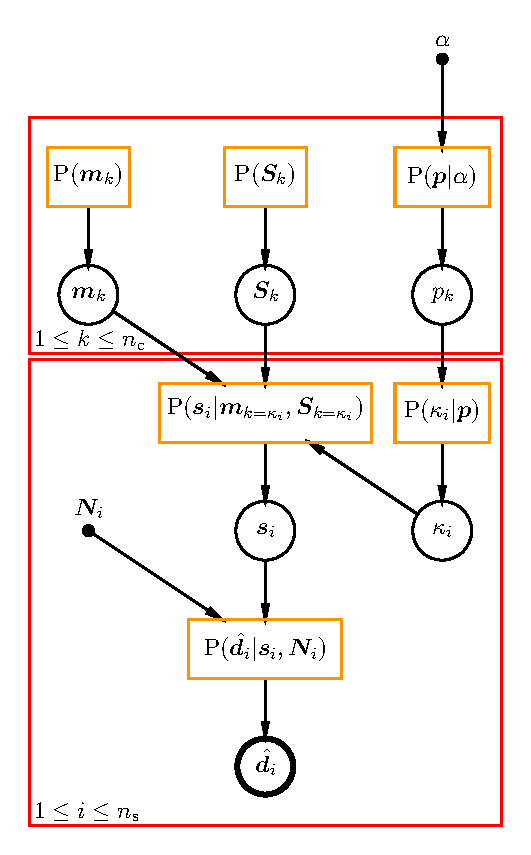
\includegraphics[width=\columnwidth]{bhm_plot.pdf}
    \caption{Network diagram for our hierarchical Bayesian model which is a graphical representation of our implemented modeling of the data. See Table 1 for the parameter descriptions.}
    \label{fig:network_diagram}
\end{figure}

For clarity, we set out our model's parameters, data and constants in Table~\ref{tab:params} and the probability distributions defining each link in the top section of Table.~\ref{tab:prob_dists}. The particular set of probability distributions chosen allow for the conditional distributions of each model parameter to be written analytically: these conditional distributions are specified in the bottom section of Table.~\ref{tab:prob_dists}. We are therefore able to use Gibbs sampling~\citep{Geman_and_Geman:1984} to estimate the joint posterior. Gibbs sampling is a special case of Metropolis-Hastings Monte Carlo~\citep{Hastings:1970} in which a single iteration consists of redrawing each parameter in turn from its conditional distribution based on the current state of the sampler. For example, in our case, we first update the class probabilities, then the class memberships, the true spectra, and finally each class's mean spectrum and covariance matrix. Drawing proposed updates from the conditional distributions means the acceptance probability is, by definition, unity, yielding a highly efficient sampler even in  high-dimensional settings. The resulting sampler is written in Python and made publicly available on Github.\footnote{\href{https://github.com/sfeeney/ddspectra}{https://github.com/sfeeney/ddspectra}}

\begin{table}
    \centering
    \caption{Model parameters, data and constants.}
    \label{tab:params}
    \begin{tabular}{ll}
        \hline
        quantity & description \\
        \hline
        $\ns$ & number of stars (29502) \\
        $\nc$ & number of classes (default: 1) \\
        $\nb$ & number of spectral bins (default: 343) \\
        $\specmean_k$ & mean spectrum of $k^{\rm th}$ class \\
        $\speccov_k$ & intrinsic spectral covariance of $k^{\rm th}$ class \\
        $\classprob_k$ & $k^{\rm th}$ class probability: fraction of stars in $k^{\rm th}$ class \\
        $\alpha$ & concentration parameter of Dirichlet prior on \\
         & class fractions \\
        $\objspec_i$ & true spectrum of $i^{\rm th}$ star \\
        $\objclass_i$ & class assignment of $i^{\rm th}$ star \\
        $\objdata_i$ & observed spectrum of $i^{\rm th}$ star \\
        $\objnoise_i$ & noise covariance matrix of $i^{\rm th}$ star \\
        \hline
    \end{tabular}
\end{table}


\begin{table*}
    \centering
    \caption{Priors, likelihoods and conditional distributions for Gibbs sampling. In our simplified notation, $\uniform$, $\dirichlet$, $\normal$ and $\invwish$ denote uniform, Dirichlet, normal and inverse-Wishart distributions, respectively.}
    \label{tab:prob_dists}
    \begin{tabular}{lll}
        \hline
        distribution & form & process \\
        \hline
        $\prob\left(\specmean_k\right)$ & $\uniform\left(-\infty,\infty\right)$ & Prior on $k^{\rm th}$ class's mean spectrum \\
        $\prob\left(\speccov_k\right)$ & $\left| \speccov \right|^{-\left(\nb+1\right)/2}$ & Prior on $k^{\rm th}$ class's spectrum covariance \\
        $\prob\left(\classprobs|\alpha\right)$ & $\dirichlet\left(\alpha\right)$ & Prior on class probabilities \\
        $\prob\left(\objspec_i|\specmean,\speccov,\objclass_i\right)$ & $\normal\left(\specmean_{k=\objclass_i},\speccov_{k=\objclass_i}\right)$ & $i^{\rm th}$ object's spectrum as Gaussian Process \\
        $\prob\left(\objclass_i = k|\classprobs\right)$ & $\classprob_k$ & $i^{\rm th}$ object's class membership \\
        $\prob\left(\objdata_i|\objspec_i,\objnoise_i\right)$ & $\normal\left(\objspec_i,\objnoise_i\right)$ & Noisy, masked spectral measurements \\
        \hline
        $\prob\left(\specmean_k | \speccov_k, \objspec, \objclasses \right)$ & $\normal \left( \frac{1}{n_k} \sum_{\objclass_i = k} \objspec_i, \frac{1}{n_k} \speccov_k \right)$ & Conditional of $k^{\rm th}$ class's mean spectrum \\
%        $\prob\left(\speccov_k | \specmean_k, \objspec, \objclasses \right)$ & $\left| \speccov_k \right|^{-(n_k + \nb + 1)/2} \exp \left( -\frac{1}{2} {\rm tr} \left[ \scalemat_k \speccov_k^{-1} \right] \right)$, where & Conditional of $k^{\rm th}$ class's spectrum covariance \\
        $\prob\left(\speccov_k | \specmean_k, \objspec, \objclasses \right)$ & $\invwish \left(n_k, \scalemat_k \right)$, & Conditional of $k^{\rm th}$ class's spectrum covariance \\
         & where  $\scalemat_k = \sum_{\objclass_i = k} \left( \objspec_i - \specmean_k \right) \otimes \left( \objspec_i - \specmean_k \right)$ & \\
        $\prob\left(\classprob_k | \objclasses, \alpha\right)$ & $\dirichlet\left(\alphas\right)$, where $a_k = \alpha + n_k$ & Conditional of class probabilities \\
        $\prob \left( \objspec_i | \specmean_{k=\objclass_i}, \speccov_{k=\objclass_i}, \objdata_i, \objnoise_i \right)$ & $\normal \left( \wfmean_i, \wfcov_i \right)$, & Conditional of $i^{\rm th}$ object's spectrum \\
         & where $\wfcov_i = \left( \speccov_{k=\objclass_i}^{-1} + \objnoise_i^{-1} \right)^{-1}$ &  \\
         & and $\wfmean_i = \wfcov_i \left( \speccov_{k=\objclass_i}^{-1} \specmean_{k=\objclass_i} + \objnoise_i^{-1} \objdata_i \right)$ &  \\
        $\prob \left( \objclass_i = k | \specmean, \speccov, \classprobs \right)$ & $ \frac{ \exp \left( -\frac{1}{2} \left[ \chi^2_{i,k} + \ln \left| \speccov_k \right| \right] + \ln \classprob_k \right) }{ \sum_{k^\prime} \exp \left( -\frac{1}{2} \left[ \chi^2_{i,k^\prime} + \ln \left| \speccov_{k^\prime} \right| \right] + \ln \classprob_{k^\prime} \right) }$, & Conditional of $i^{\rm th}$ object's class membership \\
         & where $\chi^2_{i,k} = \left( \objspec_i - \specmean_k \right)^T \speccov_k^{-1} \left( \objspec_i - \specmean_k \right) $ &  \\
        \hline
    \end{tabular}
\end{table*}

%%%%%%%%%%%%%%%%%%%%%%%%%%%%%%%%%%%%%%%%%%%%%%%%%%

%%%%%%%%%%%%%%%%%%%%%%%%%%%%%%%%%%%%%%%%%%%%%%%%%%

\section{Results}
\label{sec:results}

\subsection{Validation of Methodology: Predicting Unmeasured Spectral Regions}
\label{sec:validation}

To avoid the complications of comparing data gathered by different spectrographs, we validate our model and code by artificially masking a portion of one of our APOGEE spectra, namely the 15789 \AA\ cerium (Ce II) window of our lowest-SNR star (2M18335753-1302240), with an SNR measurement of SNR = 21 as listed in the APOGEE allStar file. We chose this feature in particular as it is a high-value detection in the APOGEE spectral region, being an s-process element and only measured for a very small subset of the APOGEE stars to date \citep{Cunha2017}. This identification and the subsequent validation of the prospect of making measurements from this line has added the prospect of examining the s-process enrichment in the APOGEE survey, building on its reach and power in mapping the alpha, light and iron-peak elements across the disk and into the halo and local group \citep[e.g.,][]{Majewski2017, Nidever2014, Hayden2015, Weinberg2019}. Nine windows were identified in \citet{Cunha2017}: we select one (unblended) Ce II window here (the line centered on 15784.75 \AA\ in air, converted to the vacuum scale of the APOGEE spectra) for validation of our methodology. 


The measured data for this star in the artificially masked region are plotted in Figure~\ref{fig:recovery_test} as a solid black line. The 68\% credible interval for the posterior probability on the star's true spectrum is plotted as dark grey, with the corresponding prediction for the observed spectrum (which also takes into account the [known] uncertainty on the observations) plotted in light grey. This prediction (strictly speaking, the posterior predictive distribution of the measured data) is in excellent agreement with the measured data, indicating that our model is capable of in-painting masked regions without bias. Note, in addition, that the uncertainty on the true spectrum is much smaller than the measurement noise, demonstrating our method's ability to de-noise observed spectra by sharing information between stars (a phenomenon known as {\it shrinkage}~\citep[see, e.g.,][Chapter 13]{Busemeyer_etal:2015}).

This de-noising property is relevant in the regime of extracting information from both weak lines and lower signal-to-noise data than typically required. In addition to the neutron capture element, Ce, the APOGEE spectral region has been shown to contain a number of r-process neodymium (Nd II) lines, which~\citet{Hasselquist_etal:2016} estimates are detectable in $\approx$ 18 percent of APOGEE spectra using equivalent width fitting techniques. Our expectation is this fraction will greatly improve given our Gaussian process modeling of the spectral lines, which can fit the true spectra of stars with lower uncertainty than the measurement noise. 
%, similarly to our demonstration of the Ce line, can generate a spectral model with lower uncertainty than the measurement noise


We note that for this illustration we have selected a narrow region around a single line, for a single star, but this is generalisable to in-paint any region, around any star \bdw{do you mean "spectral line?" or "for any star?"}. The predictive power to generate the spectra from the ensemble of all other stars and given prior measured spectral regions is detailed further in Sections~\ref{sec:inference} and~\ref{sec:info}. 


\begin{figure}
	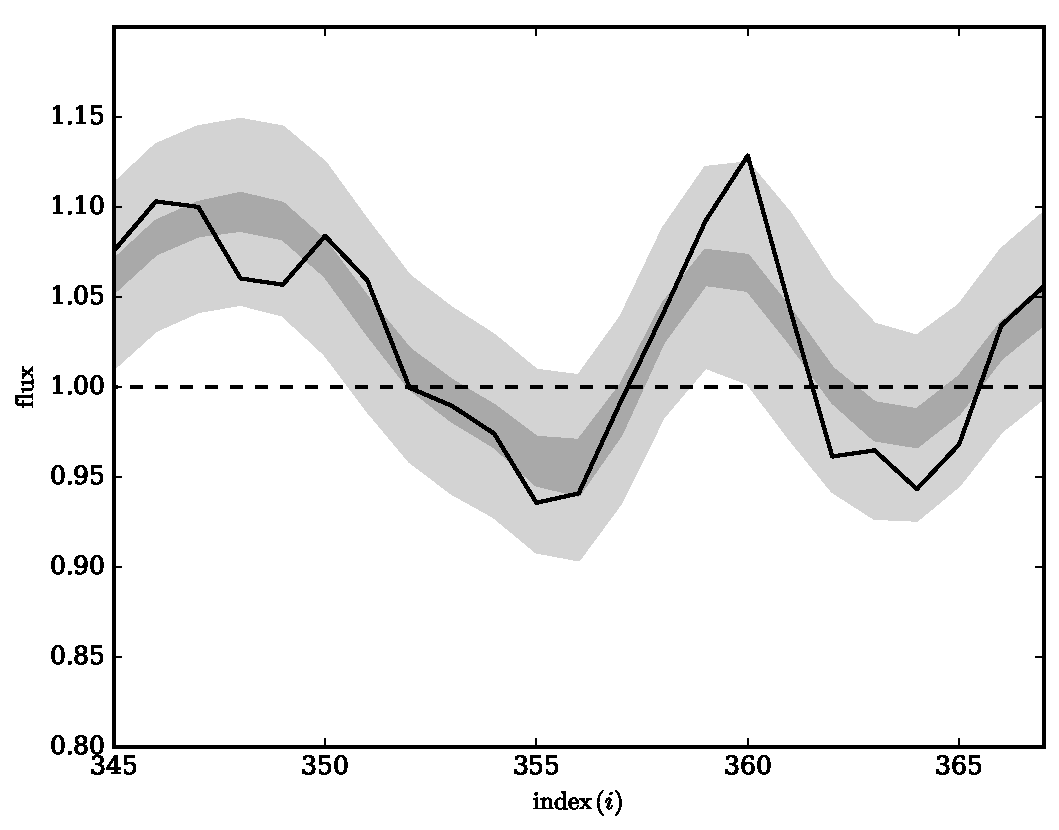
\includegraphics[width=\columnwidth]{apogee_centers_final_29502_spc_rec_test_recovery_zoom.pdf}
    \caption{This Figure demonstrates the validation of our model and method via the recovery of an artificially masked portion of one star's spectrum: a 3 \AA\ region of spectrum centred on the cerium line at 15789 \AA\ (see Table 1). We select a star with a SNR of 21 for this demonstration to highlight the performance of the model for what would traditionally be considered very low SNR data. The measured spectrum in this region is shown as a solid black line; once masked (dashed line) the flux is set to one, with infinite uncertainty. After fitting our model with the APOGEE dataset (including the remainder of this star's measured spectrum) we find that the true spectrum for this star should most likely fall in the dark grey region, and the measured spectrum (i.e., including instrumental noise) should fall in the light grey region. This is in excellent agreement with the data.}
    \label{fig:recovery_test}
\end{figure}

\subsection{APOGEE Inference: Feature Correlations Across the Abundance Windows}
\label{sec:inference}


Our inference produces samples of the probability, mean spectrum and covariance matrix for each class considered, and the true spectrum and class membership of each object. Focusing initially on the single-class case, we plot our covariance and mean inference in Figures~\ref{fig:inferred_cov} and~\ref{fig:gp_reals}, respectively. We plot the mean-posterior covariance matrix in Figure~\ref{fig:inferred_cov} (left panel). The covariance has strong off-diagonal structure, indicating that certain spectral features are highly correlated and anti-correlated. Its eigenspectrum also decays rapidly: only 241 of 557 eigenmodes have eigenvalues larger than 1/100 of the maximum. A low-rank approximation to the mean covariance retaining only these eigenmodes is plotted in the centre panel of Figure~\ref{fig:inferred_cov}, and the resulting residuals (multiplied by a factor of 500 to render visible) in the right panel. Exploiting this decaying eigenspectrum by assuming the covariance is rank deficient would greatly reduce computation time (by a factor of roughly 12 if 241 modes were retained). The most na\"ive method of reducing the covariance's rank is to project the data onto the largest $m < \nb$ principal components of the sample covariance matrix prior to inference. 

Unfortunately, \bdw{discussing this in such close proximity to the previous point can be confusing: the figure shows the inferred \textit{signal} covariance, whereas this discussion of pre-compression refers to the sample covariance of the data; I think this is a technical point that could be moved to a short subsection in the discussion on "computational considerations."} as the sample covariance contains both noise and signal its principal components are suboptimal for this task, severely degrading the inference. Modifying the hierarchical model (along the lines of \citet{Zhang_etal:2013}) to explicitly infer a rank-deficient covariance matrix is left to future work.\footnote{The structure of the covariance matrix also implies that certain kernels could potentially serve as useful covariance functions. Exploration of the utility of, for example, rational quadratic, Gibbs or mixtures of covariance functions~\citep{Rasmussen_Williams} is also left to future work.}

\begin{figure*}
	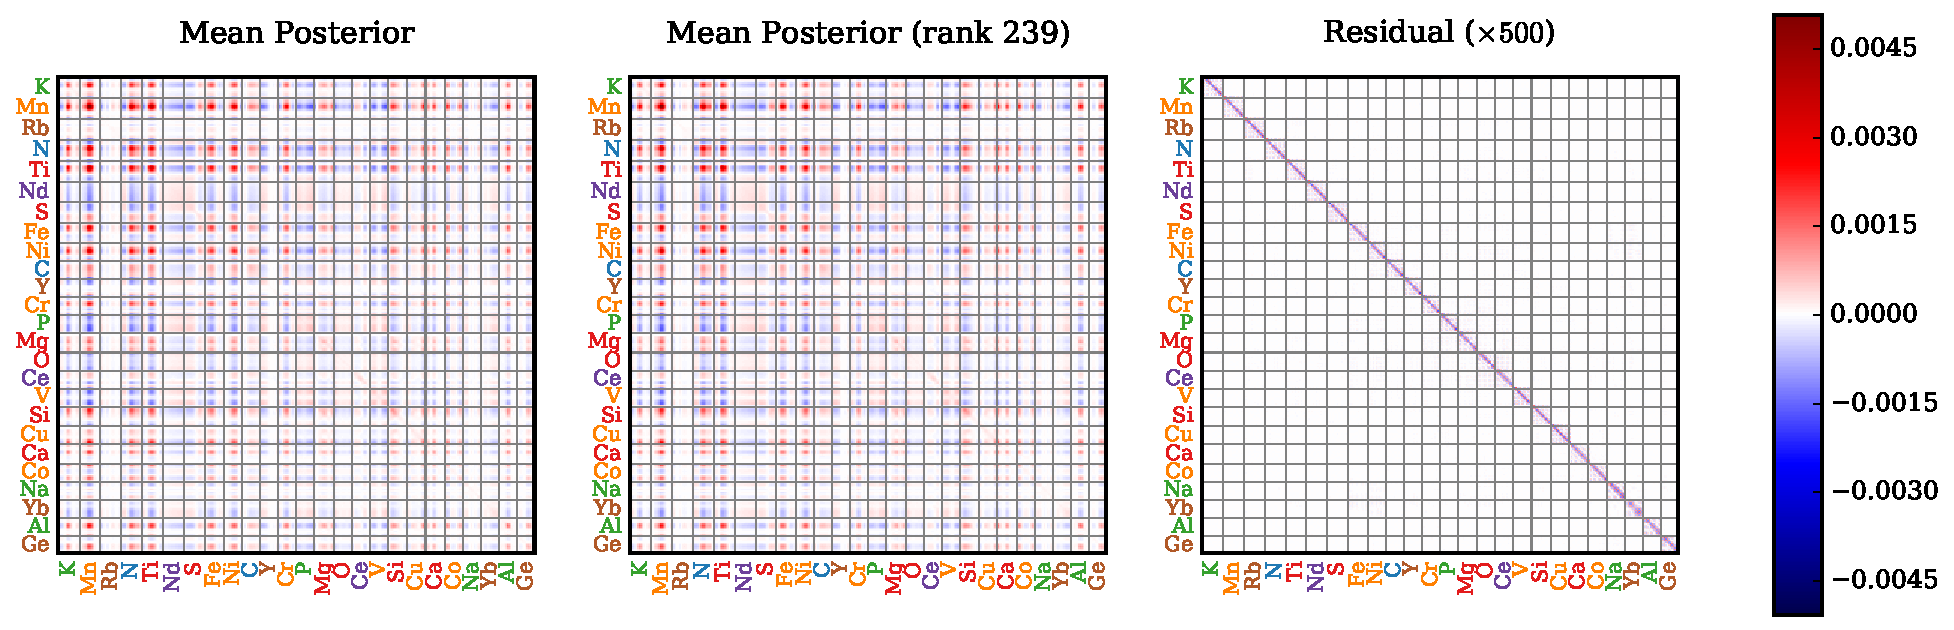
\includegraphics[width=2\columnwidth]{apogee_centers_final_29502_spc_win_wid_1p5_low_rank_covariance.pdf}
    \caption{Left: the mean-posterior covariance matrix ($\speccov$) of the 343 spectral pixels that we model, with the corresponding colour bar giving the magnitude of this covariance (in units of flux$^2$). The divergent colour map shows the most positive and negative covariances in red and blue respectively and zero covariance as white. This matrix demonstrates that the spectral pixels are highly correlated. Centre: a reduced-rank approximation of the mean-posterior covariance matrix, constructed using only those eigenvectors with eigenvalues within $10^{-4}$ of the largest. This represents a 30 percent reduction in the number of eigenvectors used to construct the mean-posterior covariance matrix. Right: the residual between the mean-posterior covariance matrix and its reduced-rank approximation, boosted by a factor of 500. The near-diagonal nature of the residuals indicates that the low-rank approximation cannot capture the additional (non-measurement) variance present in our mean-posterior covariance.}
    \label{fig:inferred_cov}
\end{figure*}
% to try to demonstrate how many 
% can speed things up in the inference by reducing the rank of the covariance matrix which is a 30 percent reduction in the number of pixels. 
%reduced rank puts null modes in the matrix - all structure in residuals is india
% the low rank version is missing variance on the diagonal 

\begin{figure*}
	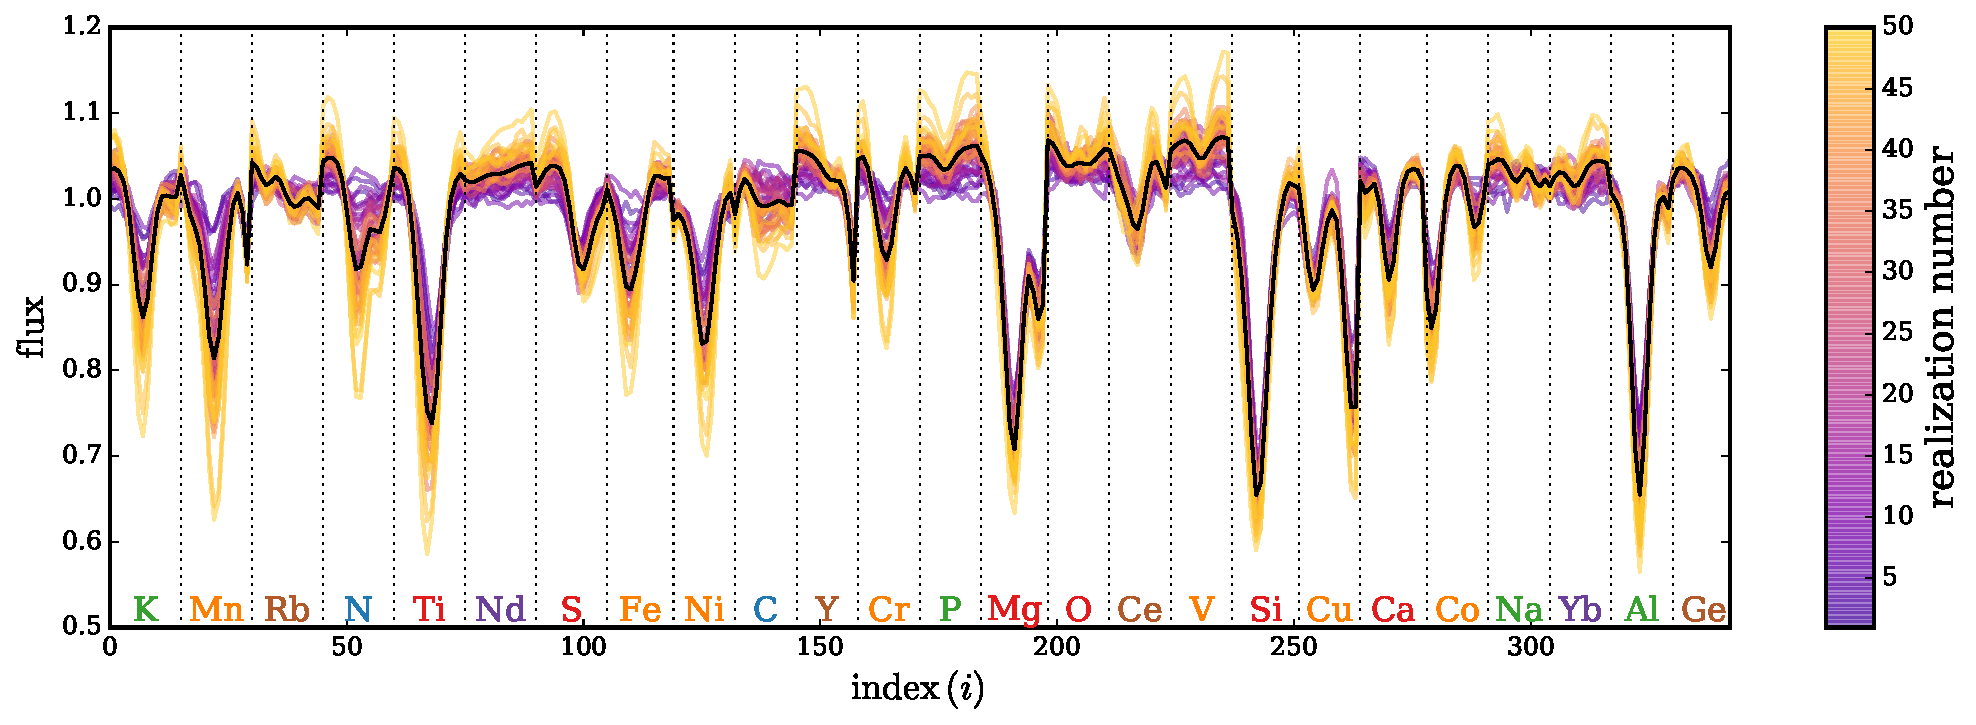
\includegraphics[width=2\columnwidth]{apogee_centers_final_29502_spc_win_wid_1p5_gp_realizations.pdf}
    \caption{The mean-posterior mean spectrum ($\specmean$) of our Gaussian process model fit using the APOGEE data (black), along with 50 random realizations of potential true spectra ($\objspec$). These draws are coloured from purple to yellow according to their flux in the first spectral bin, and serve to demonstrate the correlations between pixels. Entirely uncorrelated data would show no structure in the colour gradient beyond the first bin; however, we see a clear stratification of yellow to purple as a function of the flux magnitude for most of the pixels.}
    \label{fig:gp_reals}
\end{figure*}

%using samples of covariance matrix and samples of sample posterior you can draw examples of the spectra itself 
%samples of mean and covariance and pick a randomly chosen sample and draw a realisation of that Gaussian process from that mean and covariance. 
%mean spectrum m (posterior) and some covariance s and then have samples of those; black ine is the sum over i of the m/i 
%realisations are gaussian with mean of mi and covafaince si) 
%m$_i$, s$_i$, \specmean = \frac{\sum{i=1}{n}}{m_i}{n}; r $\sim$ N(\specmean_i, \speccov_i) 
%\specmean\ and \speccov

The posterior mean of the mean spectrum is plotted in black in Figure~\ref{fig:gp_reals}. The mean spectrum is extremely well constrained: its 68\% credible interval is narrower than the width of the line. To illustrate the covariance structure captured by our model, we overlay 50 realizations drawn from our Gaussian process model conditioned on the APOGEE data, colour-coded by the value they take in the first spectral bin. These samples can be interpreted as examples of potential noiseless true spectra that could have led to the data. They illustrate the variability permitted by the model and highlight certain clear trends, most notably highly correlated differences in line depths.

We demonstrate our inference of the true spectra of individual stars in Figure~\ref{fig:inpainting_denoising_examples}, selecting six illustrative examples. From top to bottom, we pick out two spectra whose 15789 \AA\ cerium windows are completely masked; two spectra whose 15372 \AA\ neodymium windows are fully masked; and the two lowest signal-to-noise spectra. The APOGEE IDs for these stars are 2M00014650+7009328, 2M00031631+0042234, 2M04480027+3337594, 2M06053121-0631412, 2M18335753-1302240 and 2M18295507-0340512, with signal-to-noise ratios of SNR = 49, 63, 75, 41, 21 and 23, respectively. Each panel of Figure~\ref{fig:inpainting_denoising_examples} contains two shaded regions. The pink shaded area indicates the 1-$\sigma$ deviations from the measured spectra due to noise (these are infinitely wide when the spectrum is masked); the grey, the 68\% posterior credible intervals on the true spectra. Recall \bdw{This is a technical detail that I would remove here because it breaks the narrative flow; perhaps a footnote or move to the discussion.} that we are inferring the true spectra at the measured spectral bins only. In this sense the smooth grey curves are perhaps misleading, as the posterior uncertainty is strictly infinite between data points.

Figure~\ref{fig:inpainting_denoising_examples} clearly demonstrates our ability to inpaint masked regions of spectra and denoise low signal-to-noise spectra. The inpainting results for the cerium window are particularly encouraging. We are able to make precise (and very different) estimates of these two stars' spectra in the region of the cerium line, permitting, in principle, measurements of their cerium abundances where none was previously possible. The same is true for, for example, for the aluminium lines of the third, fourth and fifth stars, along with the oxygen and germanium lines of the second, fifth and sixth stars. While we are also able to successfully inpaint the neodymium windows for the third and fourth stars, our model infers very weak line profiles in both cases, making an abundance measurement challenging. Our ability to denoise the spectra is obvious for all stars considered: the uncertainties on the true spectra are in all cases smaller than the measurement uncertainty, permitting higher-precision abundance determination than previously possible. The Sodium line of the last two stars is a particularly good example of the potential for our method to denoise spectra.

The results presented up to this point assume that the APOGEE red clump stars belong to a single class (and their true spectra are therefore realizations of a single Gaussian process). We have experimented with allowing multiple classes, initializing the sampler with random class memberships; however, we find little impact on our final results. The sampler finds slight differences between the classes' mean spectra ($\specmean_k$) and covariances ($\speccov_k$), but these are driven by the initial randomized class memberships: very few stars leave one class for another during the sampling process, and those that do typically do so only once, in the sampler's first iteration. This is because the probability distribution used for drawing a star's class membership (Table~\ref{tab:prob_dists}, last row) drops exponentially with the squared distance between the star's true spectrum and each class's mean spectrum\footnote{Specifically, the Mahalanobis distance, or number of ``sigma'' the star's spectrum is from the class's mean.}. In very high dimensions, for almost all stars the distance to a new class is typically much larger than the distance to the current class, and the probability of transitioning to a new class is essentially zero. As such, we believe the class assignments are \bdw{"random and hence uninteresting" -> strongly dependent on the choice of initial state of the Markov chain and hence not meaningful}. Exploring these high-dimensional clustering issues is left to future work. 

\begin{figure*}
	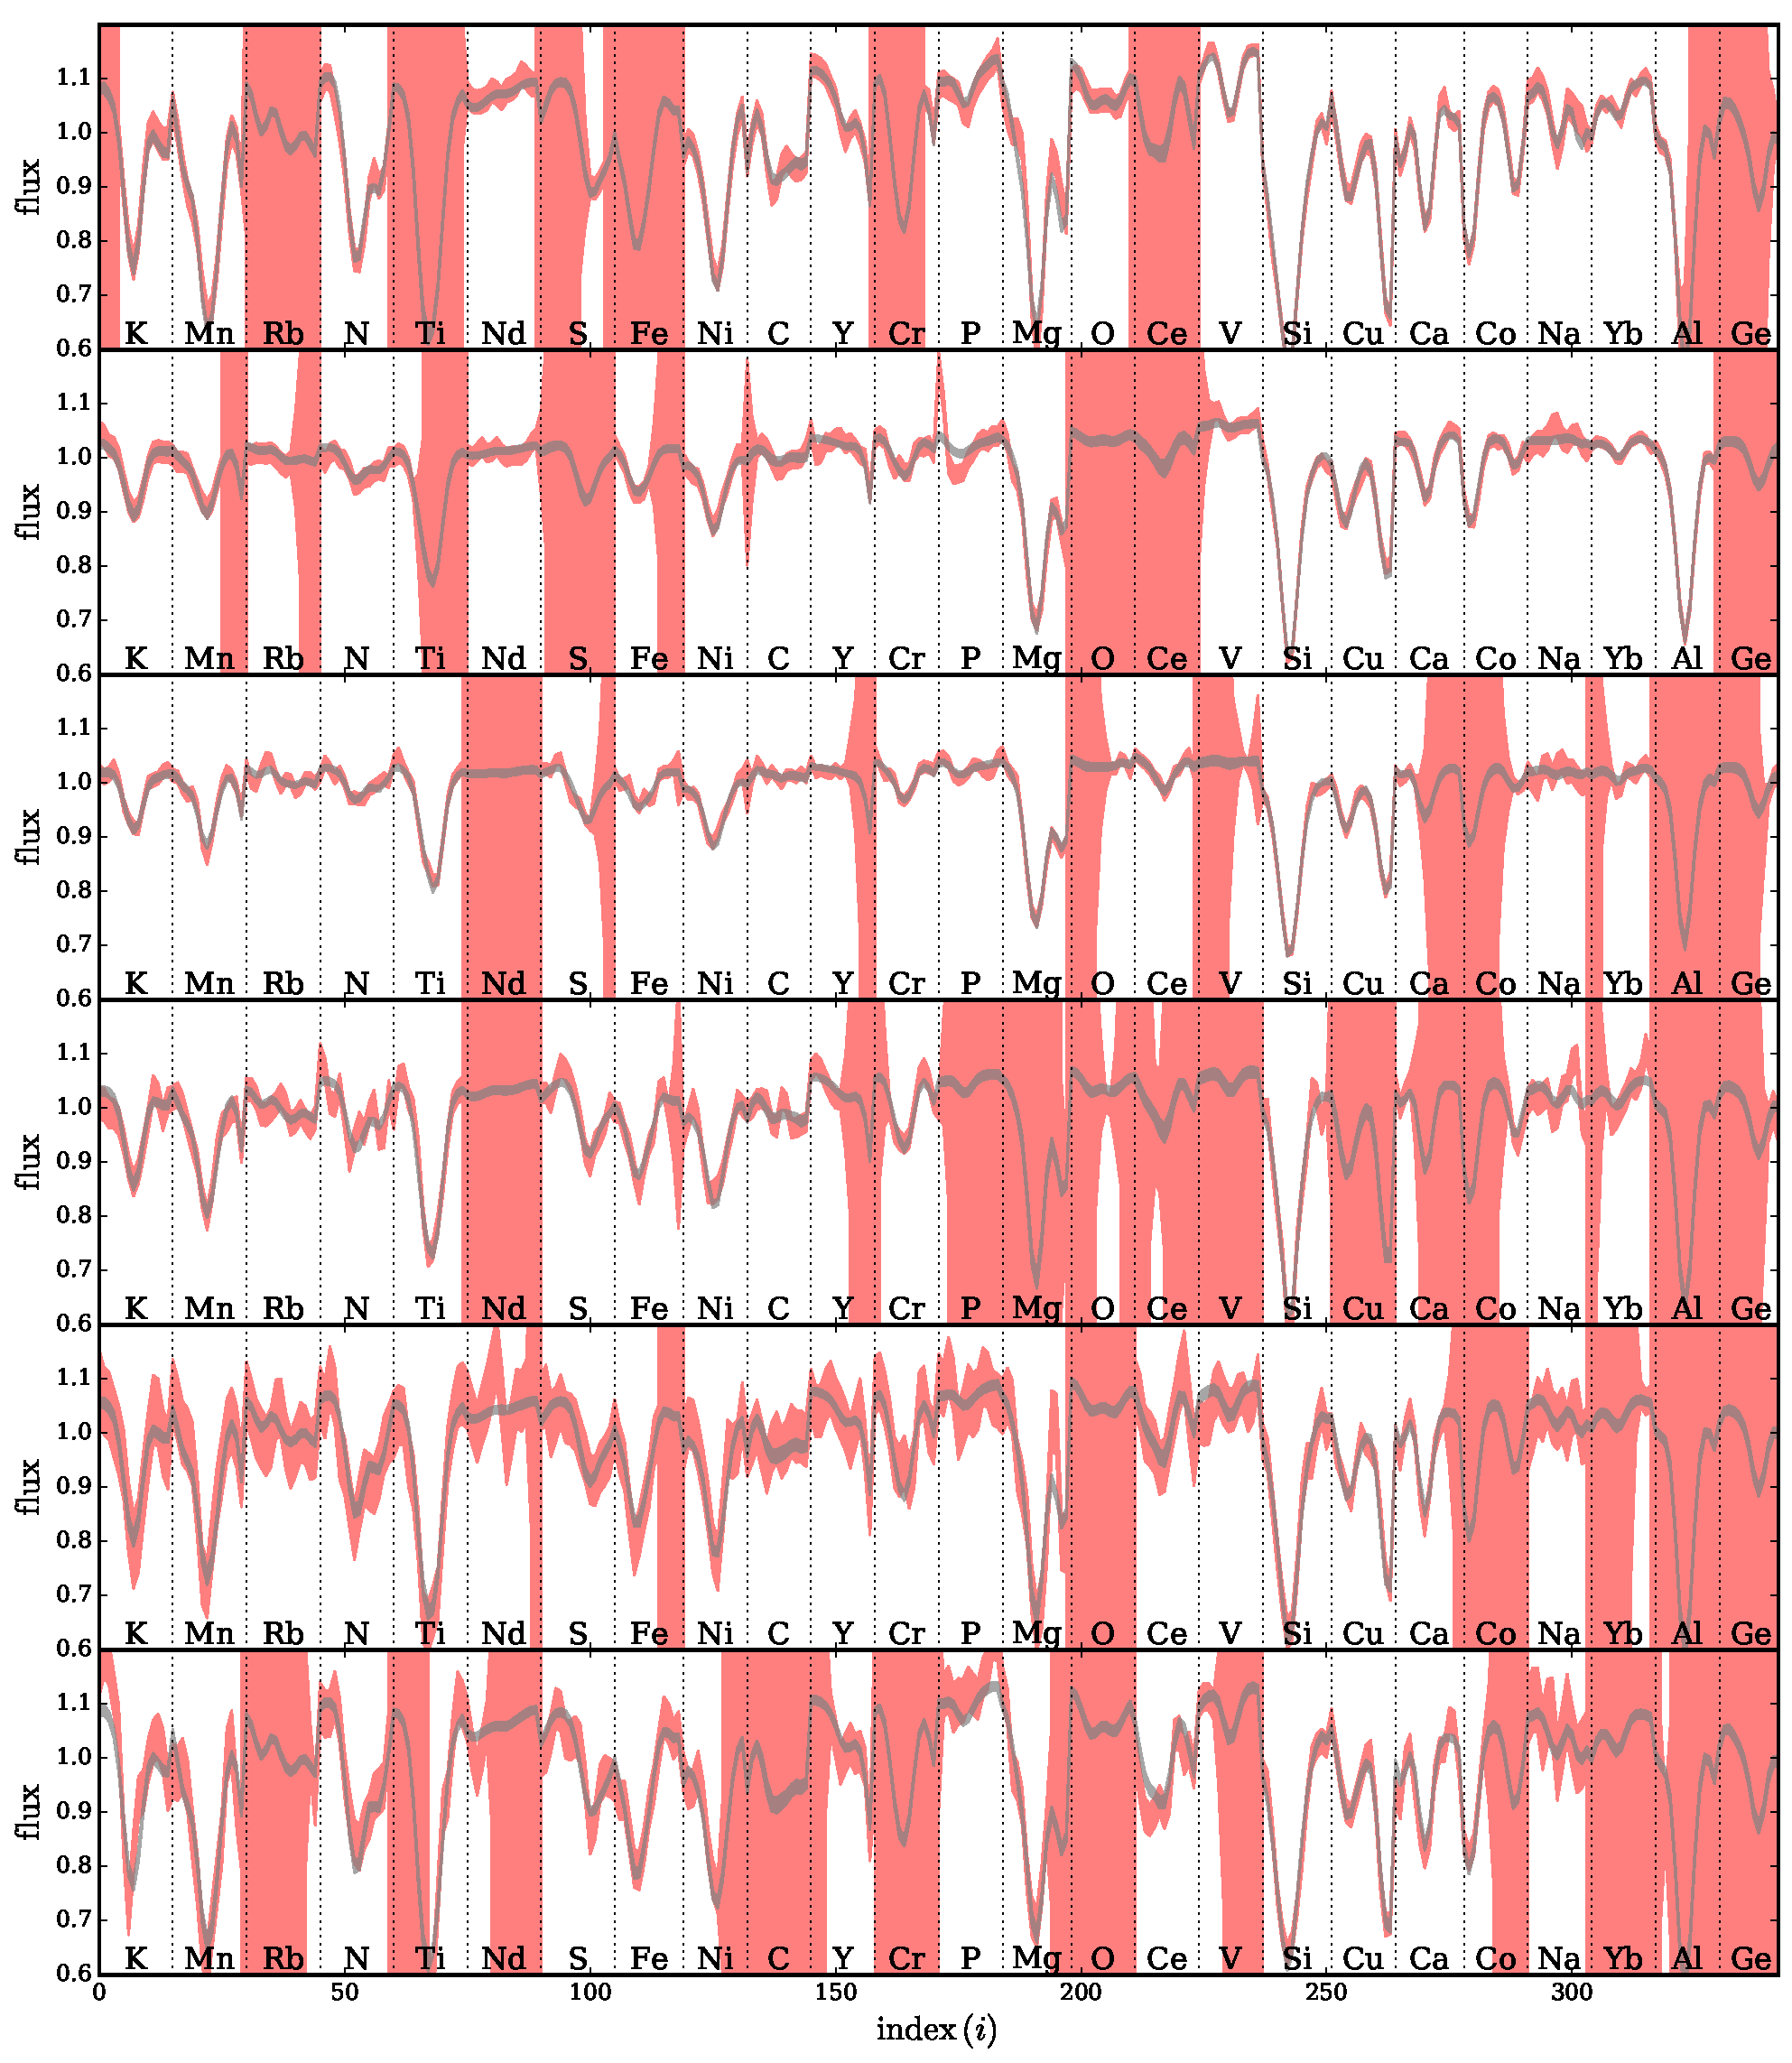
\includegraphics[width=2\columnwidth]{apogee_centers_final_29502_spc_win_wid_1p5_save_spectra.pdf}
    \caption{The measured and inferred spectra of six stars, all with low SNR (top to bottom: 49, 63, 75, 41, 21 and 23), selected to demonstrate our ability to both inpaint and denoise the data. The spectral regions shown are 3 \AA\ windows centred on the 25 elemental lines from Table~\ref{tab:window_centres}. The 68\% uncertainties on the observed spectra and inferred ``true'' spectra are shown as the pink and grey shaded regions, respectively (note the masked regions in the APOGEE spectra where the measurement uncertainties flare out to infinity). There is excellent agreement between the model and data. The first two spectra have completely masked cerium lines (15789 \AA), and the inferred spectra clearly permit the measurement of cerium abundances for these stars. The middle two stars' neodymium (15372 \AA) lines are completely masked. Though the model again inpaints these regions successfully, the resulting line profiles are very weak, rendering recovery of this abundance unlikely. All other lines inferred by the model are denoised compared to the data, permitting the estimation of higher precision abundances.}
    \label{fig:inpainting_denoising_examples}
\end{figure*}

\subsection{The Measured Information Content in the Spectra}
\label{sec:info}

We now turn to quantifying the information contained in each elemental window. Our aim is to determine the regions of spectra that are most informative about particular elements of interest. We must note, however, that our elemental windows can contain spectral features in addition to the central absorption line, and thus strong correlations between two windows are not necessarily due solely to the central elements themselves.
%, which are not absorption features of the element of interest itself. 
We start with the mean-posterior covariance within each window, $\bar{\speccov}_{XX}$, as this describes the fundamental uncertainty with which we can predict the true spectrum of a new red clump star having observed our APOGEE sample. The subscript $X$ here denotes the spectral bins defining the elemental window of interest. We summarize this covariance matrix for six elemental windows ($X=\{{\rm C, Na, Mg, Fe, Yb, Ce}\}$: one from each elemental family) by plotting the root-mean-square (RMS) uncertainty,
\begin{equation}
\bm{\sigma}_X = \sqrt{{\rm diag} \left[\bar{\speccov}_{XX}\right]},
\end{equation}
in black in Figure~\ref{fig:single_element_errs}. For context, we overlay the typical measurement uncertainty\footnote{The square root of the average noise variance in each spectral bin, where the average is taken over stars in whose spectra the bin is not masked.} as a grey dashed line. This immediately demonstrates that our model of the APOGEE spectra allows us to make sub-noise predictions for some portions of a new star's spectrum without taking further data. The results for the ytterbium window are especially interesting, as the average instrumental noise seems particularly large in this region.


\begin{figure*}
	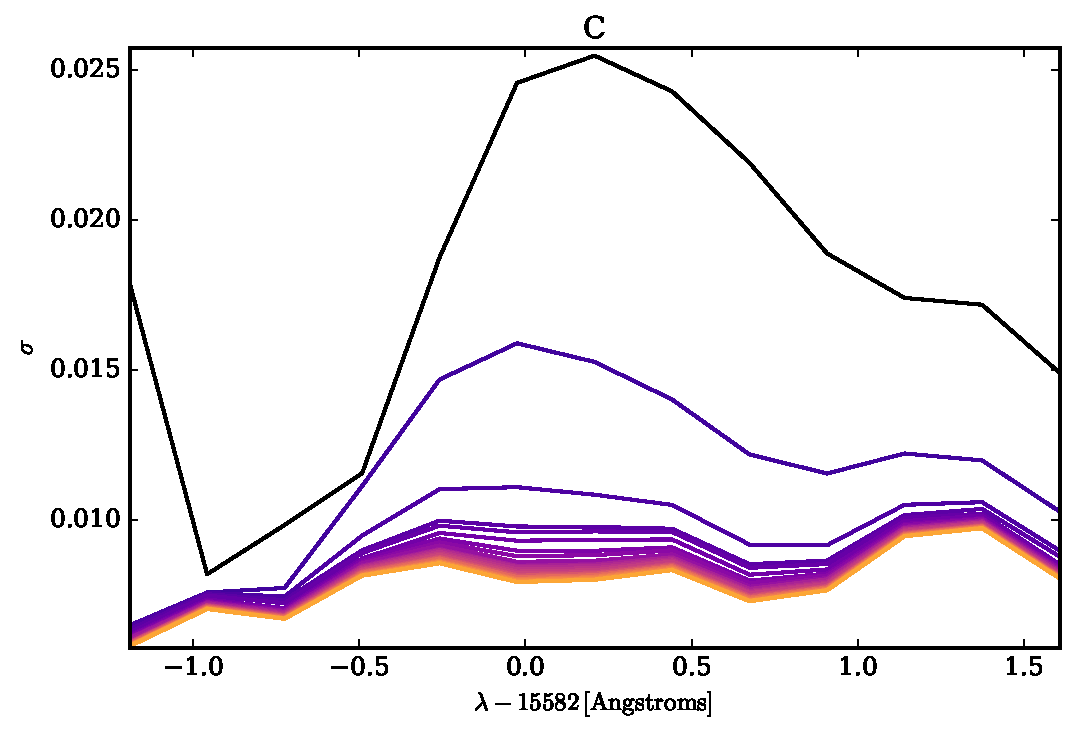
\includegraphics[width=\columnwidth]{apogee_centers_final_29502_spc_win_wid_1p5_c_conditional_stddevs.pdf}
	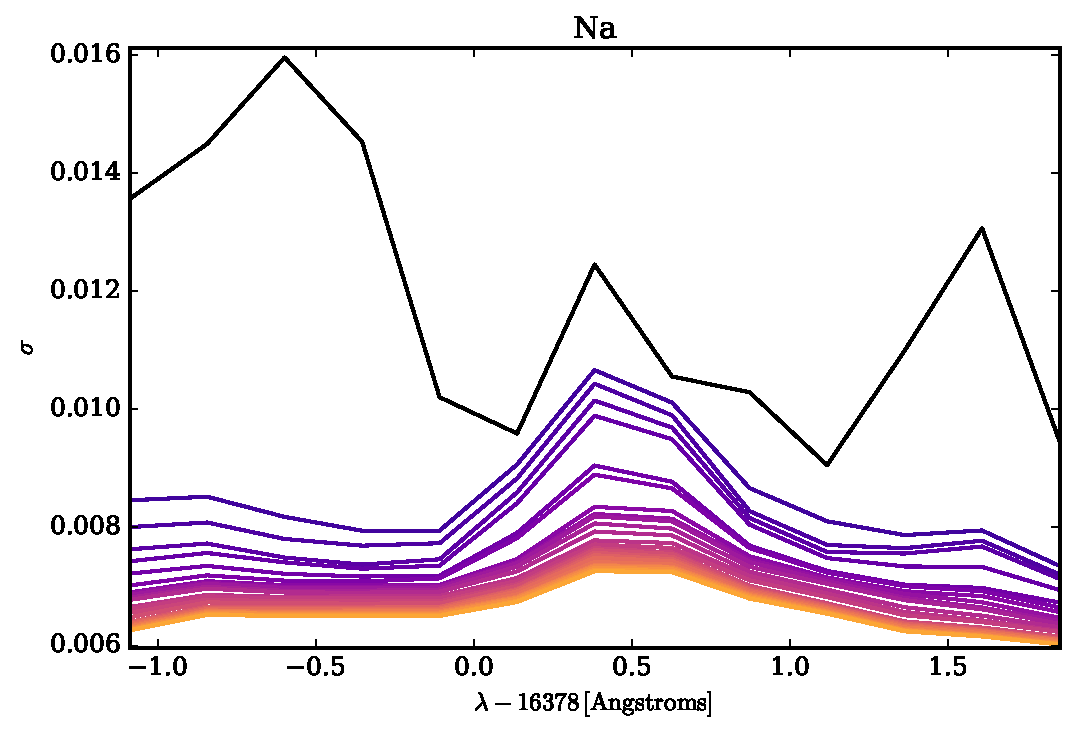
\includegraphics[width=\columnwidth]{apogee_centers_final_29502_spc_win_wid_1p5_na_conditional_stddevs.pdf}
	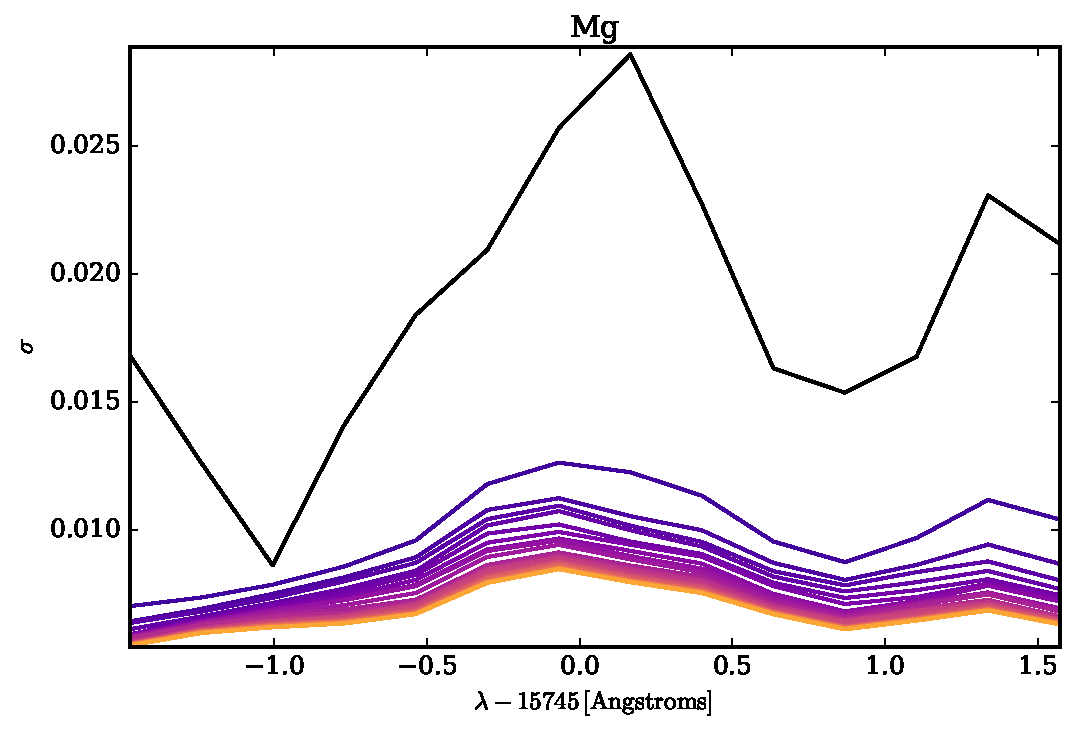
\includegraphics[width=\columnwidth]{apogee_centers_final_29502_spc_win_wid_1p5_mg_conditional_stddevs.pdf}
	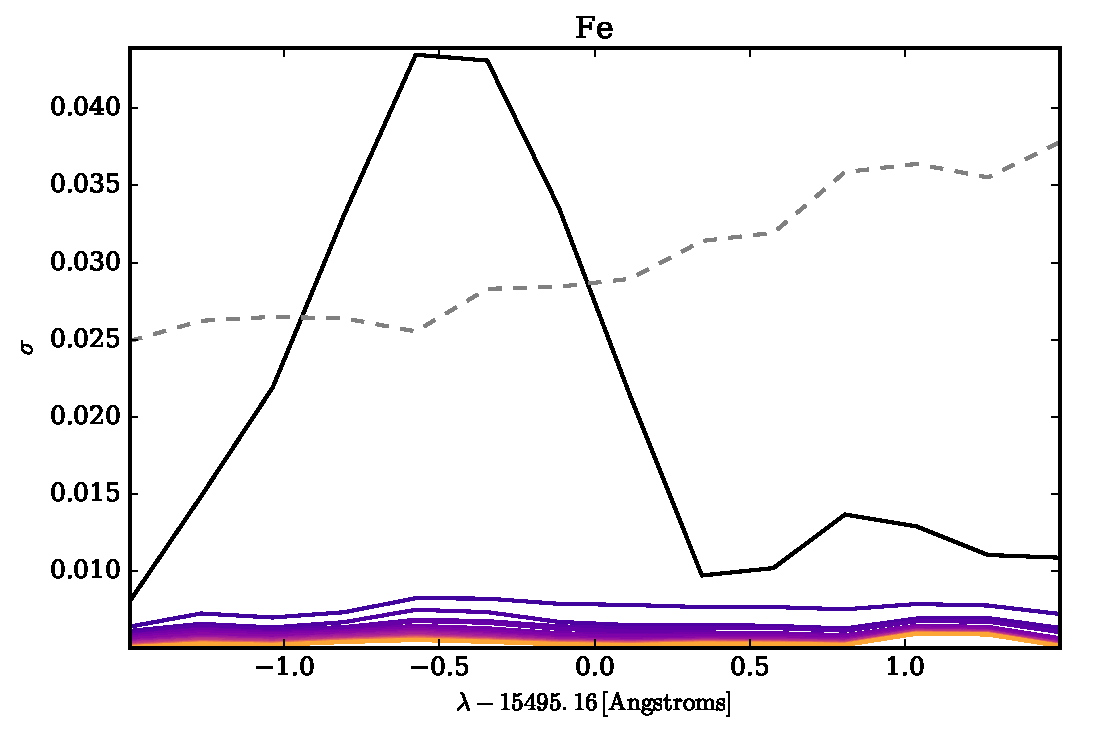
\includegraphics[width=\columnwidth]{apogee_centers_final_29502_spc_win_wid_1p5_fe_conditional_stddevs.pdf}
	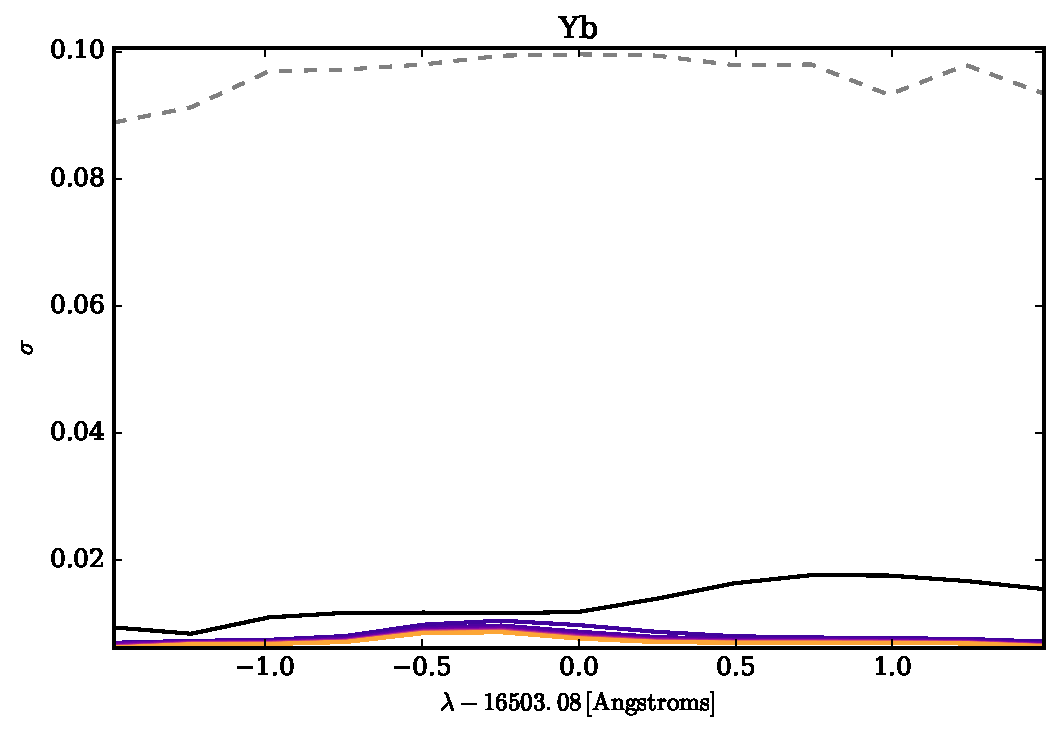
\includegraphics[width=\columnwidth]{apogee_centers_final_29502_spc_win_wid_1p5_yb_conditional_stddevs.pdf}
	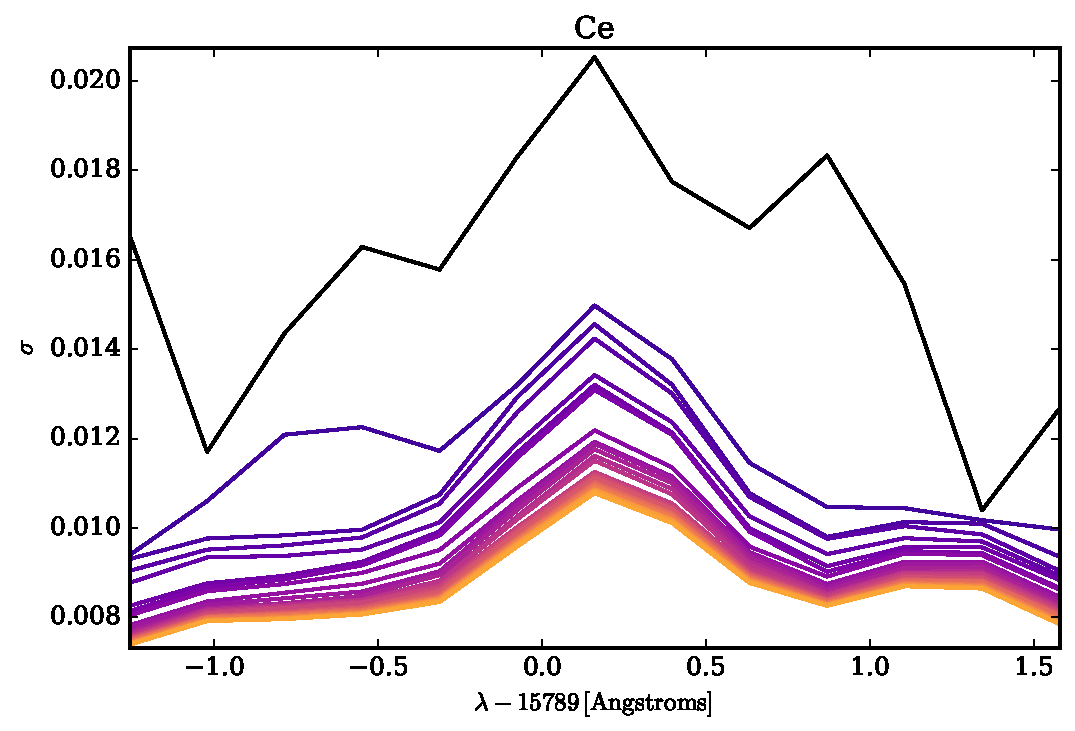
\includegraphics[width=\columnwidth]{apogee_centers_final_29502_spc_win_wid_1p5_ce_conditional_stddevs.pdf}
    \caption{Root-mean-square uncertainties on the spectra within our illustrative set of elemental windows, centred on features due to C, Na, Mg, Fe, Yb and Ce, respectively. The black line shows the uncertainty on the predicted spectrum of a new APOGEE star having not observed any portion of its spectrum; the grey dashed line indicates the typical uncertainties due to APOGEE noise. The remaining lines show how the uncertainty decreases after having perfectly observed the $1 \le n \le 24$ most informative elemental windows of the new star's spectrum, coloured from purple (most informative) to yellow (least informative). The order in which elements are added is plotted in Figure~\ref{fig:single_element_information}. Note that the impact of adding observations decreases as the information gain curves of Figure~\ref{fig:single_element_information} become less steep.}
    \label{fig:single_element_errs}
\end{figure*}


To determine which windows are the most informative, imagine observing one window of this new star's spectrum (corresponding to, say, element $Y$) {\it without measurement error}. The long-range correlations present in the inferred covariance matrix (i.e., the fact that elemental abundances are determined by a finite number of physical processes) imply that by doing so we should better constrain the elemental window of interest. To quantify the information gained about element X by (perfectly) observing element Y, we calculate the conditional covariance matrix
\begin{equation}
\condcov_{XX|Y} = \bar{\speccov}_{XX} - \bar{\speccov}_{XY} \bar{\speccov}_{YY}^{-1} \bar{\speccov}_{YX}.
\end{equation}
The conditional covariance contains our full prediction for the uncertainty on window $X$ having observed window $Y$, but we must compress it in order to construct a useful metric for quantifying information gain. We therefore define our information gain metric to be
\begin{equation}
I = \frac{1}{2} \log \frac{ \left| \speccov_{XX} \right| }{ \left| \condcov_{XX|Y} \right| } \ge 0.
\end{equation}
This can be interpreted in two ways. From an information theory perspective, the differential entropy of an $n$-dimensional multivariate normal distribution with covariance $\speccov_{XX}$ is $\frac{n}{2} \left[1 + \log 2\pi \right] + \frac{1}{2} \log |\speccov_{XX}|$~\citep[see, e.g.,][Chapter 9]{Cover_Thomas:2006}. Changing the covariance matrix to $\condcov_{XX|Y}$ as we do by observing additional windows therefore changes the differential entropy of the system (i.e., adds information to it) by precisely $I$ nats. From a geometric perspective, note that the determinant of a matrix is the hypervolume of the ellpsoid whose major axes are the eigenvectors of the matrix and have length of the eigenvalues. The square root of the determinant of a {\it covariance} matrix is therefore the volume of the error ellipsoid on the quantities of interest, up to a constant prefactor. Our metric $I$ can therefore also be interpreted as the logarithmic factor of improvement in predicting \bdw{I tightened up the  prose here}
%fractional reduction in uncertainty on
window $X$'s true spectrum obtained by observing window $Y$. Regardless of the interpretation, observing a new window can only add information, contracting the covariance matrix (or, in the worst-case scenario, leaving it unchanged), and thus $I$ cannot be less than zero.

With this metric in hand, we can take each elemental window in turn and determine the information gained by observing each other window. The window $Y^1$ with the most negative $I$ is the most informative about our target window $X$; indeed, as our metric $I$ is symmetric, these two elements are the most informative about each other. We then repeat this process, conditioning on $Y^1$ {\it and} each other window in order to find the second most informative window, $Y^2$, continuing to add windows until we find the optimal order in which to build up information on the element of interest. We denote the list of the $n$ most informative elements $\bm{Y}^n = \{ Y^1, Y^2, \ldots, Y^n \}$; the covariance in window $X$ conditioned on these elements is $\condcov_{XX|\bm{Y}^n}$.

We plot the results of this process for the six illustrative elements in Figures~\ref{fig:single_element_errs} and~\ref{fig:single_element_information}. In Figure~\ref{fig:single_element_errs} we demonstrate how the RMS uncertainty within each elemental window shrinks as we condition on more and more information, now taking the RMS uncertainty to be
\begin{equation}
\bm{\sigma}_X = \sqrt{{\rm diag} \left[\condcov_{XX|\bm{Y}^n}\right]}.
\end{equation}
We plot the RMS uncertainties after conditioning on the $1 \le n \le \nb-1$ most informative windows as a series of solid curves, coloured from purple to yellow. Observing the most informative window, $Y^1$, significantly improves the uncertainty on the spectral window of interest, and conditioning on additional windows continues to add information, albeit with diminishing returns. After observing all other windows, the RMS uncertainty at the centre of the window of interest (i.e., directly over the elemental absorption line) has been reduced by at least a factor of two for all elements bar carbon.


\begin{figure*}
	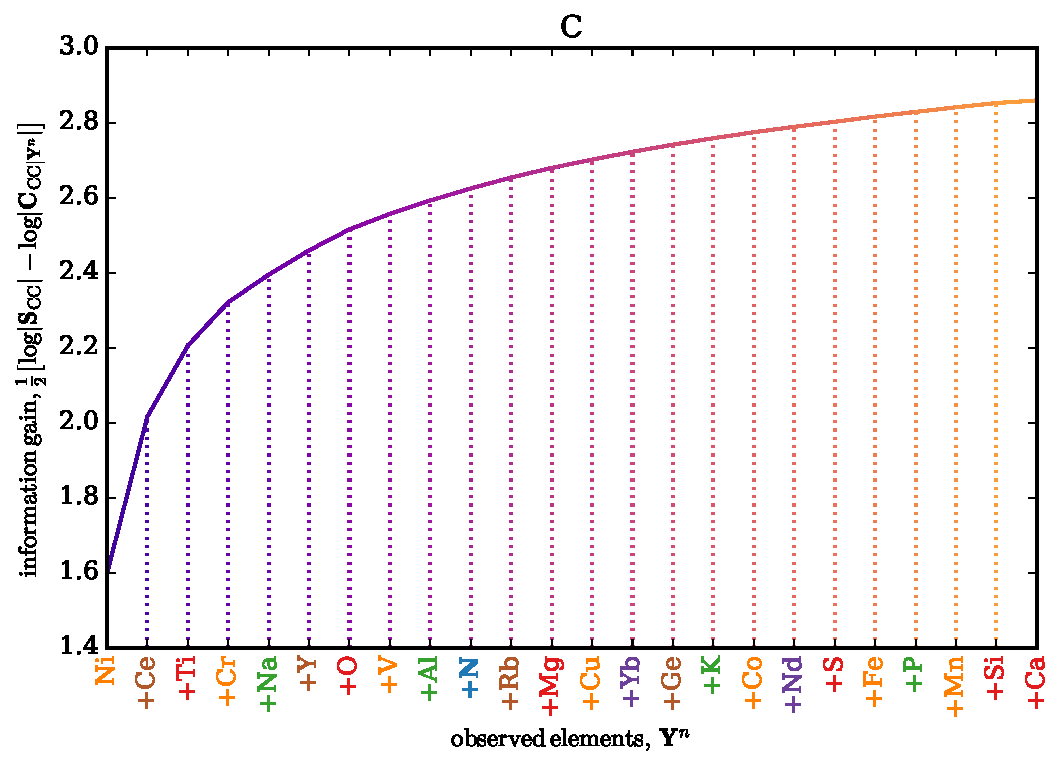
\includegraphics[width=\columnwidth]{apogee_centers_final_29502_spc_win_wid_1p5_c_inf_gain.pdf}
	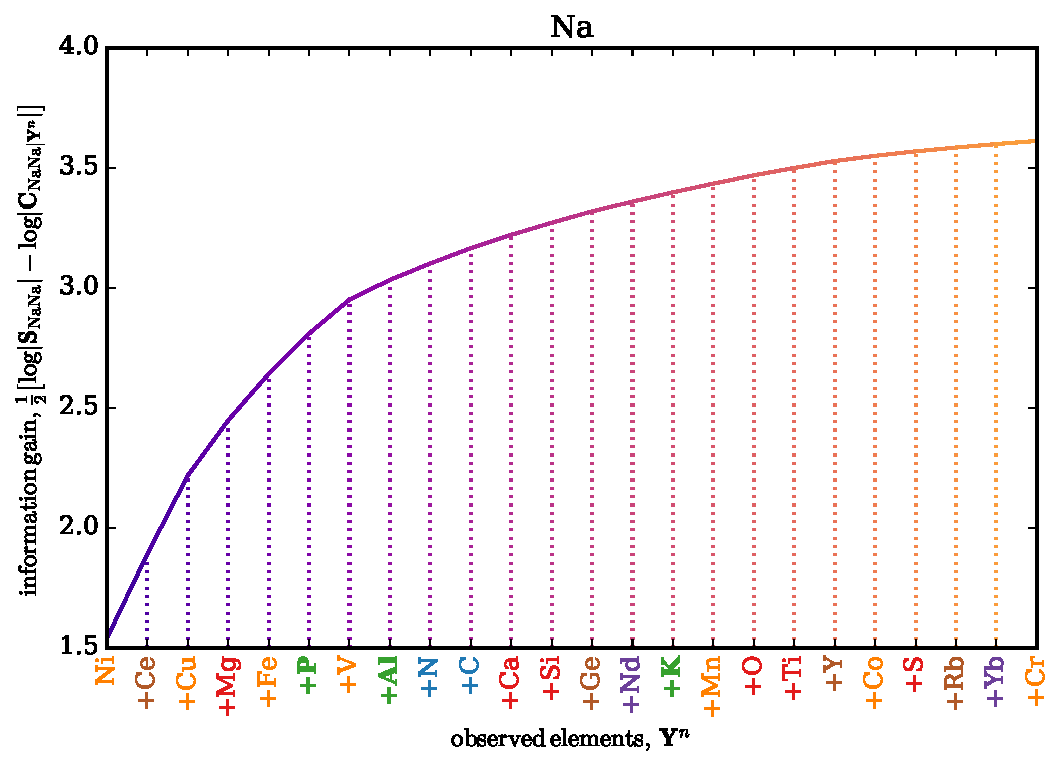
\includegraphics[width=\columnwidth]{apogee_centers_final_29502_spc_win_wid_1p5_na_inf_gain.pdf}
	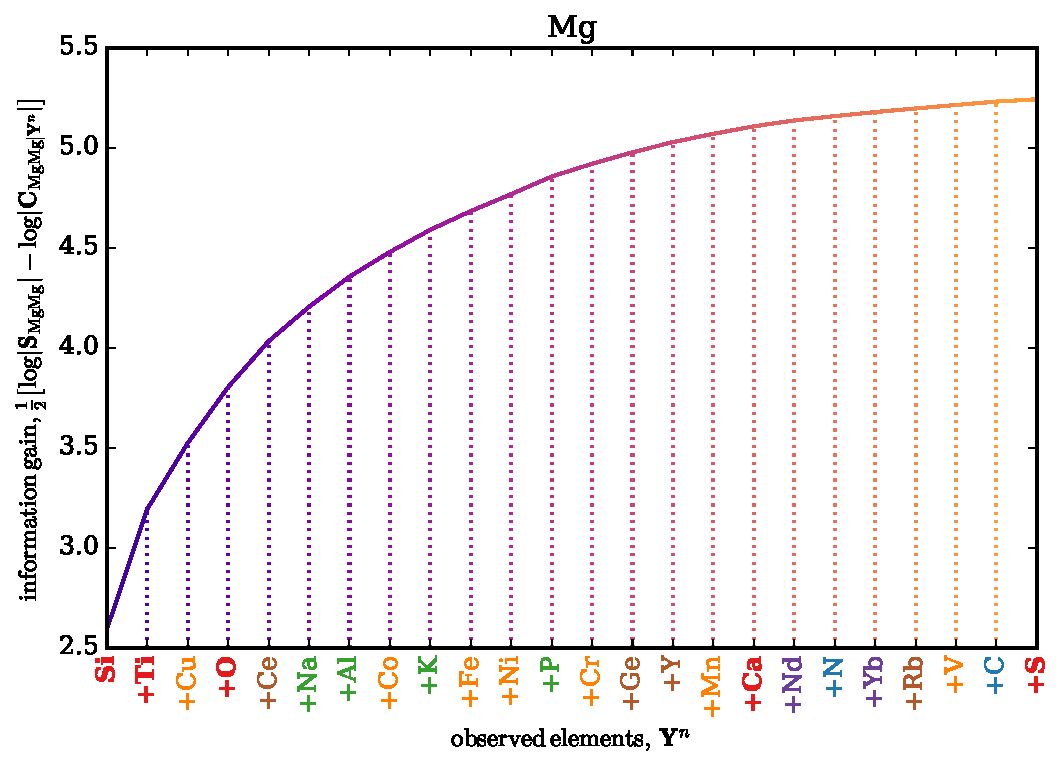
\includegraphics[width=\columnwidth]{apogee_centers_final_29502_spc_win_wid_1p5_mg_inf_gain.pdf}
	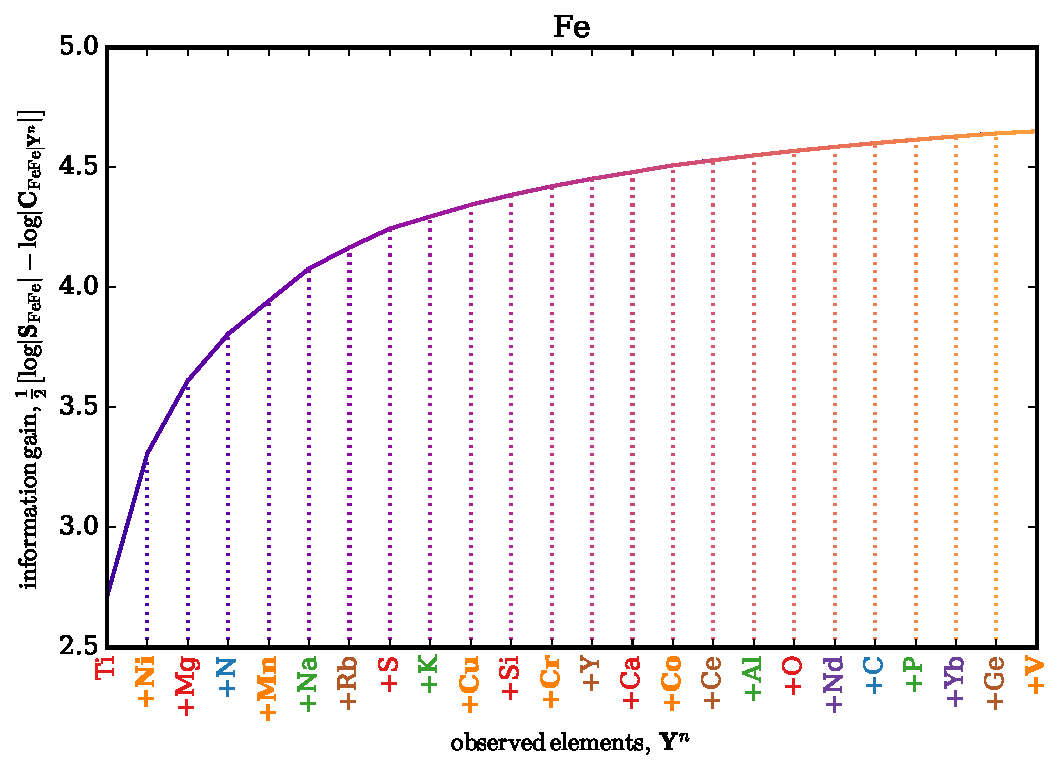
\includegraphics[width=\columnwidth]{apogee_centers_final_29502_spc_win_wid_1p5_fe_inf_gain.pdf}
	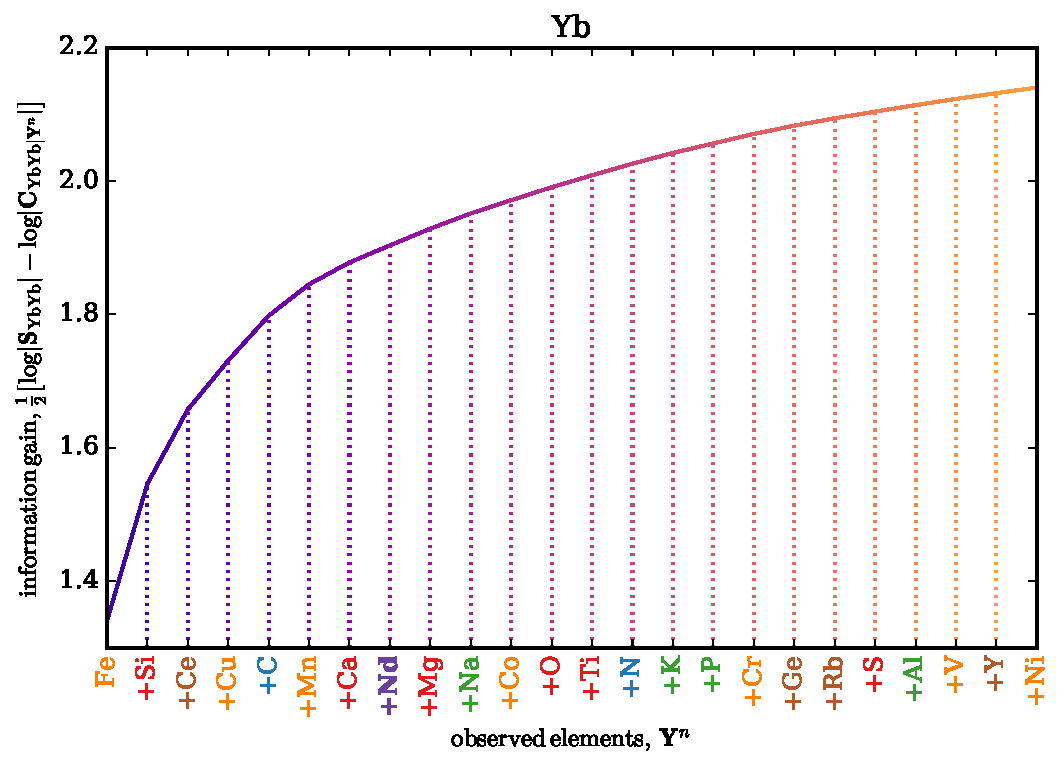
\includegraphics[width=\columnwidth]{apogee_centers_final_29502_spc_win_wid_1p5_yb_inf_gain.pdf}
	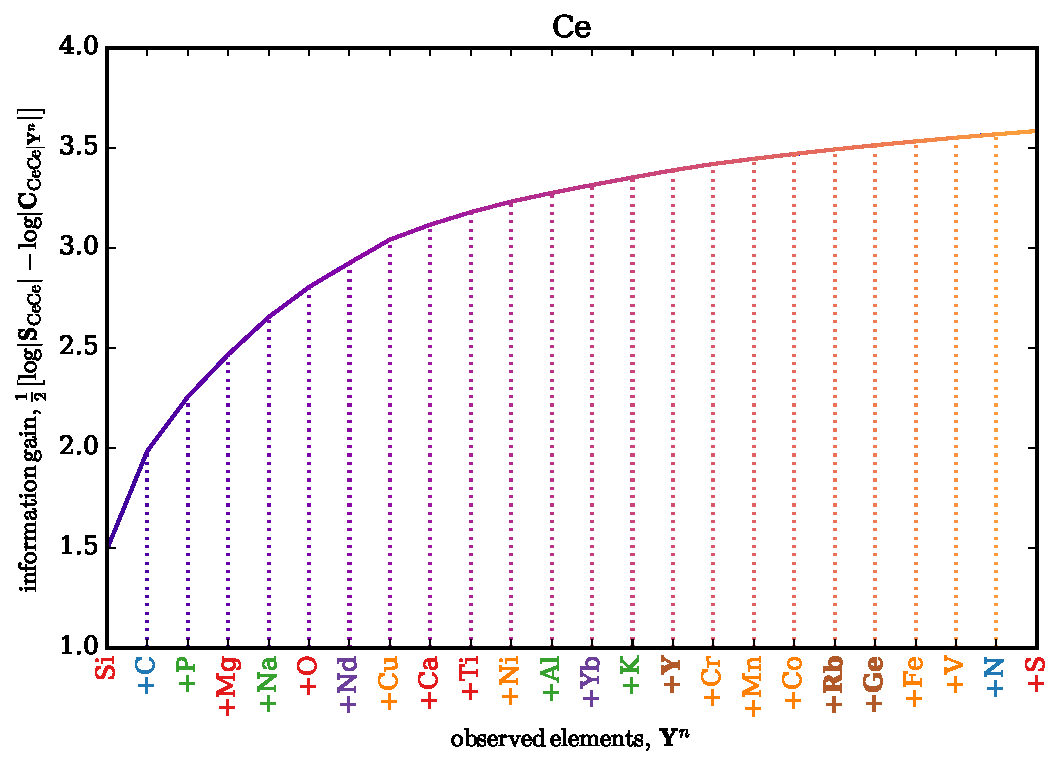
\includegraphics[width=\columnwidth]{apogee_centers_final_29502_spc_win_wid_1p5_ce_inf_gain.pdf}
    \caption{Information gains for our illustrative elemental windows obtained by observing the other 24 windows. The x-axis of each panel lists, from left to right, the window that would provide the most information on the element of interest assuming all previous windows have been observed. To take the top left-hand panel as an example: one would learn the most about the C window by observing Ni, then adding Ce, Ti, Cr {\it et cetera}. The y-axis quantifies the resulting information gain, and can be interpreted as a change in entropy of the system or the factor of reduction in the total uncertainty on the target window's predicted spectrum provided by observing the other windows. Note the different y-axis ranges for the six different elements (the most extreme being Yb and Mg): the larger the overall information gain, the better the elemental window is predicted by the rest of the spectrum. Note also that while the gain from observing successive elements decreases it does not entirely flatten: each individual element adds information on the target element. Finally, the finite range of these plots indicates that, though elements are highly correlated, no one perfectly predicts another.}
%    \caption{These set of figures represent the information gains for the windows corresponding to the elements C, Na, Mg, Fe, Ce and Ge, as shown in the top of each sub-panel, given observations of the other 24 elemental windows. Each of the element windows is shown on the x-axis, ordered from the most informative window with respect to the primary selected element, that remains after conditioning on all previous element windows. To take the top right-hand sub-panel as an example: one would learn the most about the C window by observing Ni, then adding Ce, Ti {\it et cetera}. The y-axis quantifies this predictivity of successive elements as a measure of information gain, which is the change in entropy of the system provided by conditioning on another piece of information. Note the changing range in scale of the measure of information gain for the six different elements. The gain of the 24 additional element windows in the example of the C primary window is less than the information gain for the Na primary windows. A larger overall difference is indicative of a larger overall information gain by measuring more elements. Note that the near exponential element-information gain relation, while becoming far less steep, does not entirely flatten, which indicates that each single element adds additional information to learn about the primary element. Although elements are highly correlated, there is a small intrinsic variance in each element that is not predicted in full by the remaining set of windows.}
    \label{fig:single_element_information}
\end{figure*}

% most predictive
% y axis quantifes the information gain. 
%the information gain is defined here as the difference between the log of the ratio of the determinant of the covariance matrix conditioned on observation in some other window and divided by the covariance matrix not condioned on any other obsservation. 
%log of the determinant of the covariance matirx tells  you the change in entropy of the system that you would get by conditioning on another piece of information.
% so it is very much an amoutn of information.
%low dimensional to some threshold
%two things - not looking at single elemental abundances because there might be other stuff in those windows, we are not using the same basis as abundances. Even if we were looking at abundances, not perfectly predictive. 
%intrinsic variance is coming out in this figure. 


In Figure~\ref{fig:single_element_information} we plot the most informative windows for our six elements of interest first, along with the information gained by observing each additional window moving to the right on the x-axis. The windows' labels are coloured by their elemental family, with members of the target element's family picked out in bold. Recall that our information gain metric can be interpreted as the logarithm of the fractional reduction in volume of the error ellipses on the true spectrum. These plots cover the rough range $1.4 \le I \le 5.2$, corresponding to reducing the error volume by factors of 4 to 180. Reflecting the qualitative results of Figure~\ref{fig:single_element_errs}, each of the curves in Figure~\ref{fig:single_element_information} flattens as more elements are observed, indicating that the single greatest information gain is provided by observing the most informative elemental window and the bulk of the information is provided by the first 10 or so elements. None of the curves plateau, however, and thus all elements provide information on the window of interest. It is perhaps interesting to note that the most informative element is not, in general, from the same family as the element of interest (though this is true for magnesium). We caution over-interpretation of this point, however, for two reasons: 1) this conclusion applies only to this specific set of spectral windows; and 2) these windows are broader than the elemental features they are designed to capture, and can therefore contain information about a number of elements.

%Log scale so fractional gain for first N elements is XX and fractional gain for elements $>$ 5 is XX percent, relatively independent of which element is conditioned on.

Having discussed our detailed findings for the six illustrative elemental windows, we now summarize the results for all of the elemental windows. In Figure~\ref{fig:all_element_information} we plot the information gains for every pair of windows; that is, for each elemental window we plot the information we would gain by observing each other window perfectly. As we have demonstrated in Figures~\ref{fig:single_element_errs} and~\ref{fig:single_element_information}, there is much information to be gained by adding further observations, but given there are 24! ways of ordering them we will have to make do with the first. In doing so, we at least discover the most informative elemental pairs. We present the complete set of information gains in two ways. In the left panel of Figure~\ref{fig:all_element_information}, we group the elements by their families, sorting within each family by increasing atomic number. The most informative elemental pairs (the brightest yellow pixels) are Ni-Mn (both iron-peak), Mg-Si (both alpha) and Fe-Ti (iron-peak and alpha), and this trend is generically true of the families as a whole: the iron-peak and alpha elements predict both themselves and each other well. Indeed, these elements also predict the other families well.
 

\begin{figure*}
	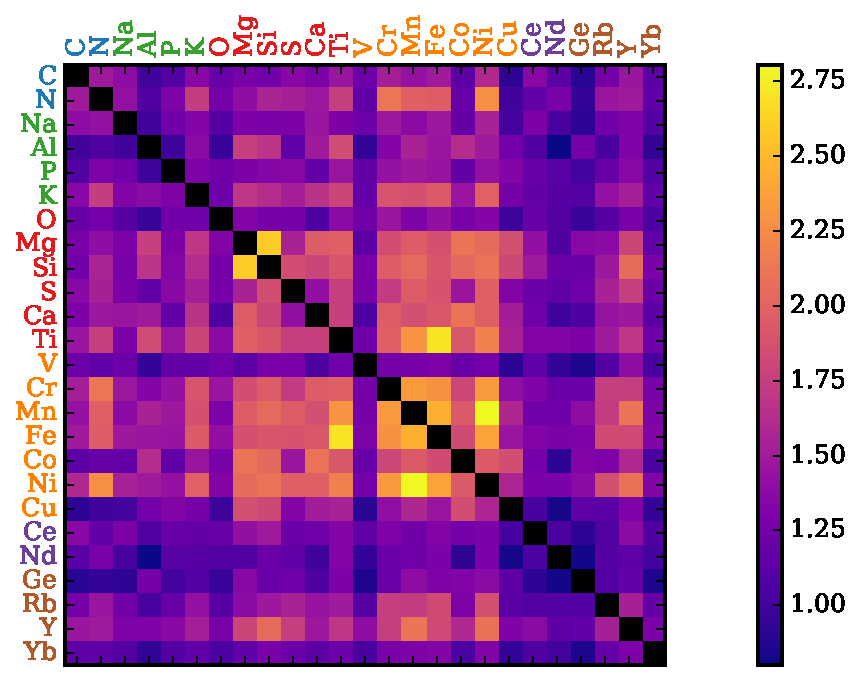
\includegraphics[width=\columnwidth]{apogee_centers_final_29502_spc_win_wid_1p5_sorted_inf_gains_fam_z.pdf}
	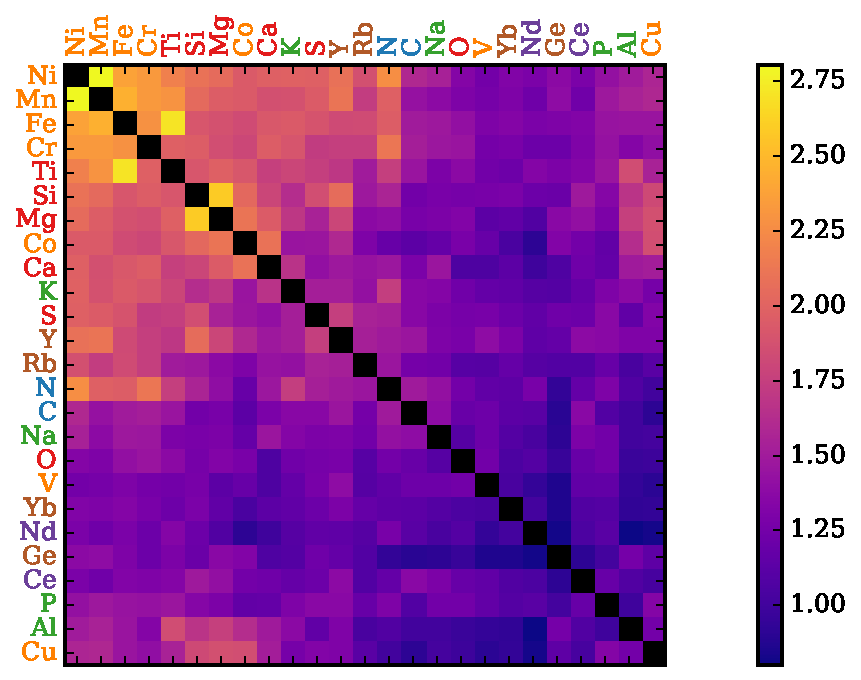
\includegraphics[width=\columnwidth]{apogee_centers_final_29502_spc_win_wid_1p5_sorted_inf_gains_abs_min_tot_dist.pdf}
    \caption{Information gains for pairs of elemental windows, colour coded from purple to yellow in order of increasing information gain. In the left panel the elemental windows are grouped according to their nucleosynthetic family, as indicated by the colour of their label. The iron-peak family of elements (and Ni, Mn, Fe and Cr in particular) are the most predictive, followed by the alpha elements (Ti, Si and Mg in particular). In the right panel, the windows are sorted to minimize the difference between adjacent rows, thereby clustering elemental windows with similar information content. Note that this does not discretely separate elements into their nucleosynthetic families, particularly beyond the iron-peak and alpha elements.}
    \label{fig:all_element_information}
\end{figure*}


There is considerable structure in this matrix, with patterns of predictivity common to multiple elements: for example, the majority of alpha-element and iron-peak rows look very similar. We make a first pass at sorting using this structure in the right panel of Figure~\ref{fig:all_element_information}. We quantify the similarity between the $i^{\rm th}$ and $j^{\rm th}$ rows in the plotted matrix of information gains using the distance
\begin{equation}
d(i \leftrightarrow j) = \sum_k |I_{ik} - I_{jk}|,
\end{equation}
where $I_{ik}$ is the information gain for the $i^{\rm th}$ element from observing the $k^{\rm th}$.\footnote{Note that we use an absolute distance metric here: using a Euclidean distance metric instead yields similar results.} To sort the elements by similar predictivity we use a simple greedy algorithm, approximating the global optimum through a series of locally optimal choices. To start, we pick an initial value of $i$, then find the most similar element by determining the row $j$ that minimizes $d(i \leftrightarrow j)$. We then take element $j$ as the comparator, calculating distances ($d(j \leftrightarrow k)$) to find the most similar of the remaining elements, and repeat until no elements remain. This approach is not guaranteed to find the global optimum, and indeed depends on the first element chosen. We therefore repeat the process with each element as the starting point and select the sorted matrix whose total distance between rows is minimal.
% define minimum distance, define sum over rows?

The resulting sorted matrix, plotted in the right panel of Figure~\ref{fig:all_element_information}, has much clearer structure than when sorted by elemental family. On the whole, the iron-peak elements are most similar as well as most predictive, closely followed by the alpha elements; copper, vanadium and oxygen are, however, notable exceptions to these patterns. There is also a fairly clean break around rubidium and nitrogen, beyond which the information gains drop noticeably. Note, however, that aluminium and copper (which are placed beyond this break) are moderately informative about titanium, silicon, magnesium and cobalt: this may well be due to the sub-optimality of the greedy algorithm.
% Determining why cobalt and calcium are so similar, for example, is something of a Time Consumer.

As cautioned above, all of the conclusions reached thus far are conditional on the precise definitions of the elemental windows set out in Table~\ref{tab:window_centres}. To gain an impression of how generic these conclusions are, we repeat the above analysis using broader, 5 \AA\ windows, presenting a version of Figure~\ref{fig:all_element_information} for these windows in Figure~\ref{fig:all_element_information_wide}. There are numerous notes to make on this Figure. First, the scale extends to larger information gains: these windows are broader, contain more features and are therefore more predictive. The choice of first element that minimizes the total distance between rows in the plot is now neodymium, not nickel, but the structure is still similar: the most informative elements are from the iron-peak and alpha group, and these elements' similar predictivities mean they cluster in the plot. There is, again, something of a drop in information gains at nitrogen; however, the iron-peak and alpha elements now predict the other families better than before. Somewhat surprisingly, for these windows Y-Ni is the most informative pair. This is, however, due to an iron line (at around 15626 \AA) that appears in the yttrium window when it is extended to 5 \AA. Finally, note that increasing the bandwidth to 5 \AA\ causes our cobalt and calcium windows to merge. These two last points serve to highlight again the fact that our conclusions derive from and apply to the full spectrum within each window, not necessarily solely to the element whose line defines the window centre. Careful consideration should be made of how to define and label windows in future work.

\begin{figure}
	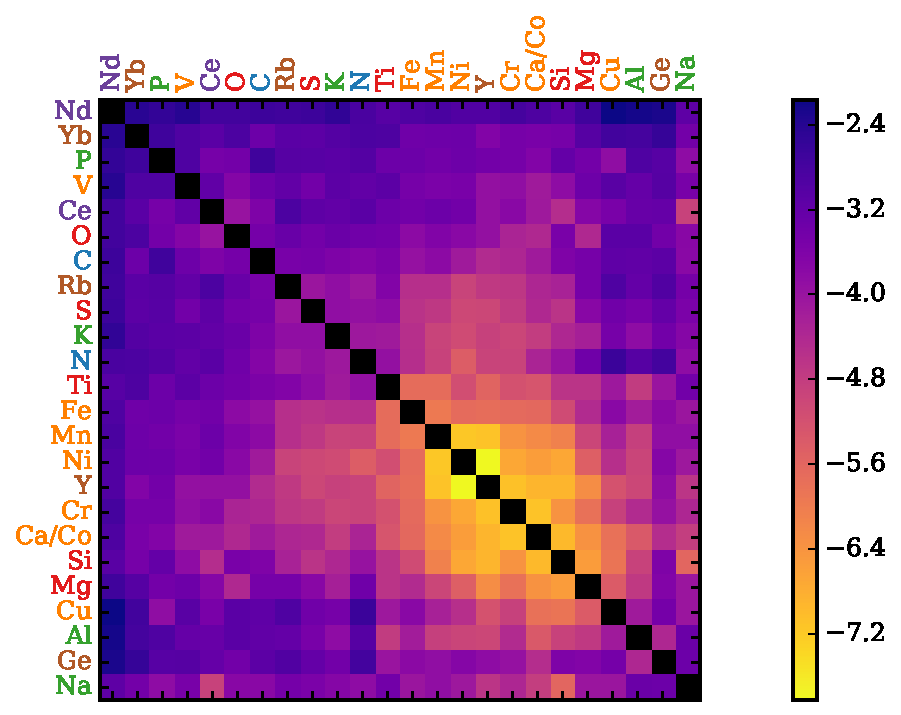
\includegraphics[width=\columnwidth]{apogee_centers_final_29502_spc_sorted_inf_gains_abs_min_tot_dist.pdf}
    \caption{Information gains for pairs of elemental windows, as in the right panel of  Figure~\ref{fig:all_element_information} (with elements grouped by similar information content), now using 5 \AA\ windows in place of our standard 3 \AA\ windows. This Figure demonstrates the impact of the precise window definitions on the information gain: the magnitude of the gains has increased and the ordering of the windows has changed, though the iron-peak and alpha elements remain most predictive and grouped as before.}
    \label{fig:all_element_information_wide}
\end{figure}

%through similarity

%%%%%%%%%%%%%%%%%%%%%%%%%%%%%%%%%%%%%%%%%%%%%%%%%%


\section{Discussion \& Conclusions}
\label{sec:discussion}

In this work, we have demonstrated how to pool information from ensembles of stellar spectra in order to denoise and inpaint individual observations with the aim of optimizing the quality and quantity of deliverables, including abundances and ages, from upcoming million-star spectroscopic surveys. We do so by modeling the distribution of 29502 APOGEE red clump stars' spectra as a high-dimensional Gaussian Process whose covariance matrix describes the variations in spectra within the population. Inferring the elements of this covariance matrix directly, we have shown that this completely data-driven model is capable of capturing the correlations between spectral pixels and harnessing them to yield improved estimates of individual spectra, along with precise {\it and} accurate predictions for unobserved spectral pixels. We produce complete spectra with decreased uncertainties for each member of the population (reducing flux errors by a factor of 2-3 for stars with SNR $\approx$ 20), enabling improved abundances to be made for all elements for every star, thereby reducing the data quality deemed necessary for precision abundance estimation. We have demonstrated our method's potential using the recently discovered 15789 \AA\ cerium line, a high-value APOGEE target due to its s-process provenance~\citep{Cunha2017}. Our model makes accurate and differentiable predictions for this line in low-SNR stars in which the line is completely masked, permitting confident measurements of cerium abundances where they would previously have not been possible.

%In the context of the million-star surveys coming online in the coming years, we seek to deliver  de-noised and ``betterized'' individual spectra for individual observations given the information we can learn from stellar ensembles. As such, we aim to optimize the quality and quantity of measurements like chemical abundances and ages that can be made from this spectra. In this work, we use an ensemble of stars to build a model that delivers de-noised individual spectra. As such, we obtain flux measurements for individual stars at higher confidence than their original observations. In Section~\ref{sec:inference}, we demonstrate the improvement in the flux uncertainty, which is a factor of $\approx$ 2 at SNR $\approx$ 20. In addition to this data uncertainty "shrinkage" we are  also able to use our model to successfully predict unmeasured regions of the spectra, that would otherwise be impossible. This enables previously unavailable features of individual stars to be measured. We achieve this using a Gaussian Process inference with multiple classes, that does not assume any analytic form for the covariance function.

%\mkn{make sure to highlight this aspect of our analysis in the text, that we show that we can denoise spectra for abundance measurements but here using the pixels themselves not isolated abundances to examine correlations and information, which is totally legitimate and useful just need to come back to this. }

% As a product of this inference, we are able to quantify the correlations and information content of the data. This interpretability of our methodology in modeling the data opens up numerous avenues of data-driven stellar charaterisation and scientific exploitation. 

Modeling the red clump stars' spectra as a Gaussian Process also allows us to quantify the information gained by observing portions of a star's spectrum, and thereby define the most mutually informative regions of spectra. We have done so for windows centred on 25 elemental absorption lines in the APOGEE wavelength range, demonstrating that the iron-peak and alpha-process elements are particularly mutually informative. While we are unable to perfectly predict the flux in any single elemental window by observing a combination of other windows, we find that the majority of information about a target window is typically contained in the 10-or-so most informative windows. This is a clear demonstration of the power of using the data themselves to drive our understanding of the diversity of (and relationships between) different nucleosynthetic channels. Indeed, the correlation structure and information content that we can measure directly should place strong constraints on the physical processes that control chemical evolution. This is relevant to founding an industry of data-driven chemical evolution models, through the assertion of the relative yields that must be obtained; yields that are currently not reproduced in detail by theoretical approaches \citep[e.g.][]{Jan2017, Blancato2019}. Our information gain results also have important repercussions for the design of future observations, motivating the targeting of carefully selected, restricted spectral windows that yield strong predictions on a range of unobserved elements.

%Our examination of the correlation between abundance windows in Section~\ref{sec:info} indicates that there is value in measuring each individual abundance. Additionally, we can say quantitatively how much value this corresponds to. Although we note, these numbers are conditioned on having observed the other spectral regions precisely. We hesitate to make strong statements at this point about the information content of individual elements, as our results are sensitive to the bandwidth of the window taken around each element absorption feature. Our general take-away's are that ..... The information content examination also demonstrates the power of using the data itself to drive our understanding of the diversity of and relationships between different nucleosynthetic channels. Indeed, the correlation structure and information content that we can measure directly should place strong constraints on the physical processes that control chemical evolution. This is relevant to founding an industry of data-driven chemical evolution models, by asserting the relative yields that must be obtained. These yields are currently not reproduced in detail from theoretical approaches \citep[e.g.][and Blancato, submitted, 2019]{Jan2017}. (because we can extract the information out quantitatively) 

It is critical at this point to address the current limitations of this method. The computational cost of the method is dominated by the matrix inversions required, which scale as the number of spectral pixels cubed. For each iteration of the Gibbs sampler we must perform one inversion per star and one inversion per class: too many for us to process the complete APOGEE dataset given available resources. In this work, we have restricted ourselves to narrow windows around our target elements; however, our results (most notably Figures~\ref{fig:single_element_information} and~\ref{fig:all_element_information_wide}) clearly show that there is significant value in including more of the spectra if possible. There are two obvious ways to achieve this: by throwing greater computational resources at the problem, or by exploiting the decaying eigenspectrum of the covariance matrices we find to infer a low-rank approximation to the covariance.

In the first approach, with access to the same number of CPUs as stars in the APOGEE sample one could reduce the number of inversions per CPU per Gibbs sample to two at most.\footnote{We must invert each class's covariance matrix in order to sample the class memberships and true stellar spectra. We must also invert the sum of each star's inverse class covariance matrix and inverse noise covariance matrix in order to update its true spectrum. While we can parallelize the loops over classes and stars, the loops must be carried out sequentially, and thus some CPUs will always perform two inversions.} Walltimes for our current 343-pixel runs are roughly 13 hours on 56 CPUs; with 29502 CPUs the full dataset could therefore be processed in 16 days, though RAM-usage considerations might also affect this calculation. While clearly computationally heavy, this is not beyond the realms of possibility for the near future, particularly considering Moore's Law. In the second approach, we have shown in this work that the simplest rank-reduction technique---namely projection of the data onto the principal components of the sample covariance matrix---fails for this dataset, indicating that a more sophisticated approach is required. The factor analysis literature doubtless contains suggestions for how to restrict the rank of the covariance and infer its structure in the resulting reduced-dimensionality space, but we leave such extensions for future work.

%\mkn{ (1) sf write... The choices specific to this data set and technical limitations are as follows......e.g. Currently limiting in this pursuit is the computational cost of the Gaussian process modeling, which here we run on a subset of APOGEE pixels. We select pixels from the full set of $\approx$ 8500 per star, which  cover 23 different element abundance absorption features. We demonstrate proof of concept and success of this approach on our subset of data.  Solving the technical challenges of feasibly scaling up to the full set of 8500 pixels for the APOGEE spectra will enable us to fully take advantage of this new era of data and the plethora of scientific exploits it enables. sf: notes for paragraphs above - other  methodological/technical aspects that would need to be further built? e.g. projection for computational cost in 5 years if nothing else changed.  }

In the meantime, we are restricted to carrying out the analysis in windows as in this work. As the results depend entirely on the windows selected, the set of windows should be carefully optimized for the task at hand. In this proof-of-concept paper, we simply selected the strongest well-defined lines for a range of interesting elements, using a fixed bandwidth for all windows. For targeted applications, our information gain metric provides a well-motivated tool with which to optimize both the positions and widths of the elemental windows used. We have demonstrated in this work that restricting to a subset of windows still permits significant denoising and inpainting, performance that will only improve through more intelligent definition of the windows; however, cutting the spectra clearly penalizes our ability to make serendipitous discoveries of new lines. We have shown here the method's ability to discover weak lines in noisy and masked spectra, but this is only possible because some stars have observed the relevant wavelengths. The loss of discovery space is a cost that must be weighed against improved performance in future applications of this work.

%\mkn{ choices - (i) we didn't optimise over any lines, we selected nominally around the strongest lines - (ii) discovery space  `` We hesitate to make strong statements at this point about the information content of individual elements, however, as our results are sensitive to the bandwidth of the window taken around each element absorption feature.''}

The final current limitation of this method is the restriction to a single class. In physical terms, this translates to the assumption that the red clump stars are distributed as a single multivariate normal in spectral space. This may be a good assumption for the red clump, but allowing for multiple classes, as discussed at the end of Section~\ref{sec:inference}, is critical in extending the scope of this first methodological demonstration beyond the red clump stars and and into the Milky Way proper. We know that different stellar populations have different spectral correlation structures: globular clusters, for example, have known abundance anti-correlations that are not seen in the disk and field halo stars~\citep[e.g.,][]{Kraft1997,Gratton2015, Pan2017,Carr2019}. It is na\"ive in the extreme to expect that all populations will have Gaussian distributions in spectral space. Modifying our sampler to correctly fit multiple classes will allow us to not only model these different, potentially non-Gaussian populations completely, but also discover new populations. This is particularly interesting as it ties into, for example, a method of understanding chemodynamical classes in the Galactic halo, which is expected to consist of discrete chemical sub-systems with different elemental correlations. Fitting multiple classes is also critical for the correct modeling and identification of outliers. Depending on their frequency, outliers will manifest as non-Gaussianity or multi-modality in the bulk population, and increase the variance of the inferred true spectra and covariance matrix if incorrectly modeled as a single Gaussian population. As with the other limitations, investigating modifications to the sampler (simulated annealing, for example) to address this issue is left to future work.

%\mkn{ sf write...something about multiple classes as we must go beyond this to generalise this approach....and include what I have written below about the fact there are different populations in the MW we know this, so this methodology not only can deal with them, but also discover them -  Dealing with them important as they exist, and discovering important as ties into i.e. a method to understand chemodynamical classes in the halo which is expected to be built of discrete chemical sub-systems with different element correlations......} The implementation of multiple classes, as discussed at the end of Section~\ref{sec:inference}, will be very relevant in expanding this first methodological demonstration beyond the red clump stars and beyond the Galactic disk. Not all stellar populations will have the same spectral correlation structure. Globular clusters for example have known abundance anti-correlations that are not seen in the disk and field halo stars \citep{}. We expect the addition of multiple classes will enable us to {\it identify} and separate populations which have distinct signatures. \mkn{currently limited by assumption in true spectrum space distribution is currently a true multivariate normal so current implementation here only good for single classes - an approximation} 
 
%\mkn{ sf: can we say something about outliers in abundances - are these handled by different classes - how would these be flagged - e.g. Li rich stars due to binary interaction? Use example of \citep{Casey2019}. Open question - resolveability can actually assign things to classes in high dimensions} 



%%%%%%%%%%%%%%%%%



 
 %refine the physical processes governing the chemical evolution of stellar systems.
 
 %\textcolor{red}{mkn: sf  - shows each have unique information but very marginal beyond some point - is it possible to state how marginal, say a factor of 100th or something like this by the time you have measured 5 elements, for pivoting on one element - do you see what I am getting at here? }

%-use this de-noised data for physics-based measuring abundances (mkn)
%-point to adding to Sloan V pipeline (mkn)
%-technical aspects of the limited number of pixels being used. cubic scaling (sf)


%\section{Conclusions}
%\label{sec:conclusions}
%-opportunity for data-driven approaches
%-this paper is first proof of concept
%-code is publicly available. 
%-successes in x,y,z, limitations in x1,y1,z1 as discussed.
%-more work to be done as outlined
%-will enable full use of the data which is going to arrive in large number for scientific exploits

%\smf{MKN: I don't feel like we need conclusions beyond the discussion but you might think differently! Let me know :)}

%-We demonstrate our methodology on the subset of 20,000 red clump stars in the APOGEE survey. Can imagine running across entire parameter space of APOGEE and providing generated model of set of abundance features for determining higher precision abundances for and where data is missing, as well as weak (Ce, Nd) elements difficult to measure from spectra. Also expect a way to classify star formation histories using correlation matricies of elements. Expect for example that a Gaussian mixture model correlation matrix of globular cluster star would look very different to field star, element correlations are direct reflection of stellar phyiscs and star formation history that is dissimilar between different Milky Way populations. Could also be used as a classifier using spectral feature correlations themselves. 
%-first characterisation / way of measuring correlation between elements/wavelength regions
%-people could use all of the de-noised regions to measure all of the interesting elements in APOGEE e.g. Ce, Nd
%Our work sets out avenues for continued exploration, and significant opportunity with respect to this is in the low resolution regime. Precision abundances can be derived from very low resolution spectra (Ho et al., 2016). We therefore must seek to better understand the information captured in the spectral features from an empirical point of view. 
%-
%- \textcolor{red}{publicly available code online here} 


%%%%%%%%%%%%%%%%%%%%%%%%%%%%%%%%%%%%%%%%%%%%%%%%%%

\section*{Acknowledgements}

The Flatiron Institute is supported by the Simons Foundation.
Melissa Ness is supported in part by the sloan Foundation. We would like to thank Brice Menard (JHU) who was instrumental in bringing our team together to perform this work. 

%%%%%%%%%%%%%%%%%%%%%%%%%%%%%%%%%%%%%%%%%%%%%%%%%%

\bibliographystyle{mnras}
\bibliography{mknbib} % if your bibtex file is called example.bib

%%%%%%%%%%%%%%%%%%%%%%%%%%%%%%%%%%%%%%%%%%%%%%%%%%


% Don't change these lines
\bsp	% typesetting comment
\label{lastpage}
\end{document}

% End of mnras_template.tex